%----------------------------------------------------------------------------------------
%	PACKAGES AND OTHER DOCUMENT CONFIGURATIONS
%----------------------------------------------------------------------------------------

\documentclass[
11pt, english, singlespacing,
%draft, % Uncomment to enable draft mode (no pictures, no links, overfull hboxes indicated)
%nolistspacing, % If the document is onehalfspacing or doublespacing, uncomment this to set spacing in lists to single
%liststotoc, % Uncomment to add the list of figures/tables/etc to the table of contents
toctotoc, % Uncomment to add the main table of contents to the table of contents
%parskip, % Uncomment to add space between paragraphs
%nohyperref, % Uncomment to not load the hyperref package
%headsepline, % Uncomment to get a line under the header
%chapterinoneline, % Uncomment to place the chapter title next to the number on one line
%consistentlayout, % Uncomment to change the layout of the declaration, abstract and acknowledgements pages to match the default layout
]{MastersDoctoralThesis}

%----------------------------------------------------------------------------------------
%	PACKAGES
%----------------------------------------------------------------------------------------
\usepackage[utf8]{inputenc} % Required for inputting international characters
\usepackage[T1]{fontenc}
\usepackage{mathpazo} % Use the Palatino font by default


%-------------------------------- Define the LIBRARY ------------------------------------

\usepackage[backend=biber,style=numeric,sorting=none,sortcites=true,style=numeric-comp]{biblatex}
\AtBeginBibliography{\renewcommand*{\finalnamedelim}{\addspace\bibstring{and}\space}}
\renewcommand*{\bibnamedash}{\ifnumgreater{\value{liststop}}{1}{\space et al.}{}} % Et al. bei mehreren Autoren
%\renewcommand*{\bibfont}{\small} % Optional: Make the bibliography font size smaller
\addbibresource{Chapters/My_bibliography.bib}
\RequireBibliographyStyle{customstyle_bibiliography} % Load the custom style
%----------------------------------------------------------------------------------------


\usepackage[autostyle=true]{csquotes}

\usepackage{hyperref}
\usepackage{amsmath, amssymb, amsfonts}
\usepackage{bm}       % For bold Greek letters
\usepackage{caption}
\captionsetup{width=1.0\textwidth, font=normal, labelfont=bf}

%----------------------------------------------------------------------------------------
%	MARGIN SETTINGS
%----------------------------------------------------------------------------------------

\geometry{
	paper=a4paper,
	inner=2cm, % Inner margin
	outer=3cm, % Outer margin
	bindingoffset=.5cm, % Binding offset
	top=1.5cm, % Top margin
	bottom=1.5cm, % Bottom margin
	%showframe, % Uncomment to show how the type block is set on the page
}

%----------------------------------------------------------------------------------------
%	THESIS INFORMATION
%----------------------------------------------------------------------------------------

\thesistitle{Subradiant routing on a Y-shaped atomic tree in free space}
\supervisor{Prof. Dr. Beatriz \textsc{Olmos Sanchez	}}
\examiner{Prof. Dr. Igor Lesanovsky}
\degree{Bachelor of Science}
\author{Leopold \textsc{Bodamer}}
\addresses{Taubenstraße 7, 72138 Kirchentellinsfurt}
\subject{Theoretical Atomic Physics and Synthetic Quantum Systems}
\university{\href{https://uni-tuebingen.de\\}{Eberhard Karls Universität Tübingen}}
\department{\href{https://uni-tuebingen.de/fakultaeten/mathematisch-naturwissenschaftliche-fakultaet/fachbereiche/physik/institute/institut-fuer-theoretische-physik/arbeitsgruppen/}{Institut für Theoretische Physik}}
\group{\href{https://uni-tuebingen.de/fakultaeten/mathematisch-naturwissenschaftliche-fakultaet/fachbereiche/physik/institute/institut-fuer-theoretische-physik/arbeitsgruppen/ag-lesanovsky/}{Theoretical Atomic Physics and Synthetic Quantum Systems}}
\faculty{\href{https://uni-tuebingen.de/fakultaeten/mathematisch-naturwissenschaftliche-fakultaet/fakultaet/}{Mathematisch-Naturwissenschaftliche Fakultät}}

\AtBeginDocument{
\hypersetup{pdftitle=\ttitle}
\hypersetup{pdfauthor=\authorname}
}

\begin{document}

\frontmatter
\pagestyle{plain}

%----------------------------------------------------------------------------------------
%	TITLE PAGE
%----------------------------------------------------------------------------------------

\begin{titlepage}
  \begin{center}
  
  %\vspace*{.06\textheight}
  {\scshape\LARGE \univname\par}\vspace{1.5cm} % University name
  %\includegraphics[scale = 0.15]{Uni_logo}\vspace{1.5cm} % University/department logo - uncomment to place it
  
  \textsc{\Large Bachelor Thesis}\\[0.5cm] % Thesis type
  
  \HRule \\[0.4cm] % Horizontal line
  {\huge \bfseries \ttitle\par}\vspace{0.4cm} % Thesis title
  
  \HRule \\[1.5cm] % Horizontal line
   
  \begin{minipage}[t]{0.4\textwidth}
  \begin{flushleft} \large
  \emph{Author:}\\
  {\authorname} % Author name
  \end{flushleft}
  \end{minipage}
  \begin{minipage}[t]{0.4\textwidth}
  \begin{flushright} \large
  \emph{Supervisor:} \\
  \href{https://sites.google.com/site/beatrizolmosphysics/}{\supname} % Supervisor name - remove the \href bracket to remove the link  
  \end{flushright}
  \end{minipage}\\[3cm]
   
  \vfill
  
  \large \textit{A thesis submitted in fulfillment of the requirements\\ for the degree of \degreename}\\[0.3cm] % University requirement text
  \textit{in }\\[0.4cm]
  \groupname\\\deptname\\[2cm] % Research group name and department name
   
  \vfill
  
  {\large \today}\\[4cm] % Date
  
  \vfill
  \end{center}
  \end{titlepage}
  
  %----------------------------------------------------------------------------------------
  %	DECLARATION PAGE
  %----------------------------------------------------------------------------------------
  
  \begin{declaration}
  \addchaptertocentry{\authorshipname} % Add the declaration to the table of contents
  \noindent I, \authorname, declare that this thesis titled, \enquote{\ttitle} and the work presented in it are my own. I confirm that:
  
  \begin{itemize} 
  \item This work was done wholly or mainly while applying for a research degree at this University.
  \item Where any part of this thesis has previously been submitted for a degree or any other qualification at this University or any other institution, this has been clearly stated.
  \item Where I have consulted the published work of others, this is always clearly attributed.
  \item Where I have quoted from the work of others, the source is always given. With the exception of such quotations, this thesis is entirely my own work.
  \item I have acknowledged all main sources of help.
  \item Where the thesis is based on work done by myself jointly with others, I have made clear exactly what was done by others and what I have contributed myself.
  \end{itemize}
   
  \noindent Signed:\\
  \rule[0.5em]{25em}{0.5pt} % This prints a line for the signature
   
  \noindent Date:\\
  \rule[0.5em]{25em}{0.5pt} % This prints a line to write the date
  \end{declaration}

%----------------------------------------------------------------------------------------
%	ABSTRACT PAGE
%----------------------------------------------------------------------------------------

\begin{abstract}
\addchaptertocentry{\abstractname}
This thesis investigates the directional routing of excitations in atomic systems using subradiant states.
Building on Bottarelli's quantum router \cite{Startingpoint}, this thesis adapts the model to atomic systems,
addressing the challenges of controlling interactions in fully connected systems.
Atom light interactions have been heavily studied for atomic lattices \cite{Masson2022, Asenjo-Garcia2017, Needham2019, Cech2023, Jen2016}.
In this theis three chains, that are connected by an equilateral triangle and an isosceles triangle are studied.
By allowing different dipole orientations on each chain, three distinct topologies are considered.
The results show that controlling the topology and the initial state enables directional routing,
where a topology with equilateral triangle and aligned dipoles emerges as the most practical for stable readout.

	
\end{abstract}
%----------------------------------------------------------------------------------------
%	CONTENTS
%----------------------------------------------------------------------------------------
\mainmatter
\pagestyle{thesis}

%----------------------------------------------------------------------------------------
%	ACKNOWLEDGEMENTS
%----------------------------------------------------------------------------------------

\begin{acknowledgements}
\addchaptertocentry{\acknowledgementname}
I would like to express my deepest gratitude to those who supported me throughout this journey.
First and foremost, I sincerely thank my supervisor \supname for her guidance and encouragement.
Her mentorship was crucial in shaping this work.

\noindent
A special thanks to Marcel Cech, whose expertise and advice greatly contributed to the development of this work.
I am also deeply grateful for my colleagues and fellow students,
Niklas Schmid, Paul Haffner, Ardit Thaqi, Christian Gommeringer for their assistance,
which made this experience both productive and enjoyable.
One of them was Richard Marquardt, who was always ready to provide mathematical help.

\noindent
I would like to especially thank Malik Jirasek, Niclas Schilling, Anna Schupeta and Paul Haffner for proofreading this thesis.
Additionally,
I am thankful to Tabea Bodamer for her assistance with English grammar and to Konstanze Bodamer for her financial support.
\noindent
Finally, I would like to extend my appreciation to my girlfriend, Anna Schupeta, for her constant love, patience,
and understanding through this process.

\end{acknowledgements}

%----------------------------------------------------------------------------------------
%	LIST OF CONTENTS/FIGURES/TABLES PAGES
%----------------------------------------------------------------------------------------

\tableofcontents % Prints the main table of contents

%\listoffigures % Prints the list of figures
%\listoftables % Prints the list of tables

%----------------------------------------------------------------------------------------
%	ABBREVIATIONS
%----------------------------------------------------------------------------------------

%\begin{abbreviations}{ll} % Include a list of abbreviations (a table of two columns)
%
%\textbf{LAH} & \textbf{L}ist \textbf{A}bbreviations \textbf{H}ere\\
%\textbf{WSF} & \textbf{W}hat (it) \textbf{S}tands \textbf{F}
%
%\end{abbreviations}

%----------------------------------------------------------------------------------------
%	PHYSICAL CONSTANTS/OTHER DEFINITIONS
%----------------------------------------------------------------------------------------

%\begin{constants}{lr@{${}={}$}l} % The list of physical constants is a three column table
%
%% The \SI{}{} command is provided by the siunitx package, see its documentation for instructions on how to use it
%
%Speed of Light & $c_{0}$ & \SI{2.99792458e8}{\meter\per\second} (exact)\\
%%Constant Name & $Symbol$ & $Constant Value$ with units\\
%
%\end{constants}

%----------------------------------------------------------------------------------------
%	SYMBOLS
%----------------------------------------------------------------------------------------

%\begin{symbols}{lll} % Include a list of Symbols (a three column table)
%
%$a$ & distance & \si{\meter} \\
%$P$ & power & \si{\watt} (\si{\joule\per\second}) \\
%%Symbol & Name & Unit \\
%
%\addlinespace % Gap to separate the Roman symbols from the Greek
%
%$\omega$ & angular frequency & \si{\radian} \\
%
%\end{symbols}














%----------------------------------------------------------------------------------------
%	DEDICATION
%----------------------------------------------------------------------------------------

%  \dedicatory{For/Dedicated to/To my\ldots}
\chapter{Introduction} % Main chapter title
\label{Chapter1} % Change X to a consecutive number; for referencing this chapter elsewhere, use \ref{ChapterX}

%----------------------------------------------------------------------------------------
%	SECTION 1
%----------------------------------------------------------------------------------------
\section{Motivation}
\noindent
Quantum computing, an exceptionally promising area of study in modern physics, offers a fundamentally new way to process and transmit information.
Applications of this, not yet scalable technology range from cryptography to drug research.
Quantum computers would especially outperform classical computers in quantum simulations of chemical / physical systems \cite{Eddins2022}.
Qubits, the analog to classical bits, for example,
photons or atoms play a crucial role in harnessing this quantum technology \cite{Ramakrishnan2023}.
The area which describes photons and their interaction with matter is quantum optics.
One essential goal of this filed is to build efficient and controllable interactions between photons and atoms.
A challenge for this is unwanted (spontaneous) emission, where photons are scattered into channels out of control.
This spontaneous emission hampers the development of quantum technologies, especially in quantum information processing.
%Quantum information processing stands at the forefront of modern technological advancement.
Subradiant states are a promising concept for this field of study.
These states appear when many emitters interact via light-mediated resonant dipole-dipole interactions
and inherit lifetimes magnitudes larger than that of a single emitter \cite{AsenjoGarcia2017}.
Insights into information transport within complex systems are of utmost interest,
as they could lead to advances in quantum computing. %routing and storage
Especially with subradiant states, as they also offer ultrafast readout \cite{Scully2015}.
%Zhen Wang et al. demonstrated, that a switching between sub- and superradiant modes is possible \cite{Wang2020}.

%----------------------------------------------------------------------------------------
%	SECTION 1
%----------------------------------------------------------------------------------------
%\section{Objective}
\vspace{0.5cm}
\noindent
The goal of this thesis is
to perform robust directional photon routing on atomic systems in free-space using subradiant states.
Focusing on a Y-shaped atomic tree, different topologies are explored to enable long-lived information transport as a proof of concept.

    \section{Outline}
This thesis is structured as follows.
Chapter \ref{Chapter2} introduces the theoretical background.
It covers the concepts of open quantum systems,
subradiance and superradiance, the Green tensor, and the reciprocal space.
These tools are essential foundations for describing atom-atom interactions in free space,
including dipole-dipole interactions and coupling to a photonic bath.
%After this chapter, the reader already knows...
The quantum router of \cite{Startingpoint} is presented and summarized in Chapter \ref{Chapter3}.
It introduces the concepts of graph theory and explains how quantum evolution on a graph topology can be utilized to achieve directional routing of information.
Chapter \ref{Chapter4} will be the core of this thesis, adapting this model to an atomic system.
This chapter delves into the challenges of implementing directional routing in a fully connected atomic system and investigates various solutions to control the phase of interactions.
It further extends the analysis to systems with a larger number of atoms, focusing on coupling control and routing capabilities in different configurations, such as equilateral and isosceles triangles.
Chapter \ref{Chapter5} concludes the thesis by summarizing the results and discussing potential future directions in the field of quantum routing in atomic systems.
\chapter{Theoretical background}
\label{Chapter2}

\noindent
This chapter introduces the theoretical foundation
for describing the dynamics in a system of $N$ atoms that interact with a radiation field.
First, the theory of open quantum systems is presented, which allows for the description of a general quantum mechanical system interacting with its environment.
Using this framework, the interaction between atoms and light can be analyzed.
An important phenomenon in this context is collective dissipation, particularly sub- and superradiance, which is explained in \autoref{sec:Coherent_Dissipation}.
Additionally, \autoref{sec:Green_tensor} introduces a mathematical tool for describing the electromagnetic field: the Green's tensor.
Now all tools are laid out to describe the open atomic system.
An effective equation for a single photonic excitation in a system of $N$ atoms is derived in \autoref{sec:Adapt_to_System}.
The evolution depends on the geometry of the system.
Finally, the chapter discusses the important example of an atomic lattice.
In this case, the analysis can be extended to the so-called reciprocal space, which enables tuning the transport properties of the excitation.
This is important for \autoref{Chapter4}, where an excitation will be transported on a topology of three connected chains.



%----------------------------------------------------------------------------------------
%	SECTION 2
%----------------------------------------------------------------------------------------
\section{\textbf{O}pen \textbf{Q}uantum \textbf{S}ystems} \label{sec:OQS}
Every real-world quantum system $\text{S}$ (except for the whole universe) is inevitably interacting with an environment/a bath $\text{B}$.
This interaction introduces additional degrees of freedom that influence the system's behavior, complicating its analysis.
An effective equation of motion, the so-called Lindblad master equation, is found for the (sub-)system of interest $\text{S}$.
Detailed derivations of this equation can be found in \cite{Breuer2002, Manzano_2020}.
The main ideas are outlined here.

\noindent
The combined Hamiltonian of the system is given by

\begin{equation} \label{eq:Hamiltonean_H_S_H_B_H_I}
\hat{H} = \hat{H}_{\text{S}} + \hat{H}_{\text{B}} + \hat{H}_{\text{I}},
\end{equation}

\noindent
where $\hat{H}_{\text{S}}$ ($\hat{H}_{\text{B}}$) act only on the Hilbert spaces of $\text{S}$ ($\text{B}$) respectively, and $\hat{H}_{\text{I}}$ describes their interaction.
In the Dirac picture, a state only evolves, according to the time-evolution operator $ \hat{U} $ with the non-interacting Hamiltonian
$\hat{H}_{\text{0}} = \hat{H}_{\text{S}} + \hat{H}_{\text{B}}$.

\noindent
A stochastic quantum state can be described by a density matrix $\hat{\rho}$.
In the Dirac (also called interaction-) picture,
the evolution of the total density matrix $\hat{\rho}$ is given by the Liouville-von Neumann equation \cite{Manzano_2020}

\begin{equation}\label{eq:Liouville_v_N}
\frac{d\hat{\rho}(t)}{dt} = -\frac{i}{\hbar}  \left[ \hat{H}'_I(t), \hat{\rho}(t) \right],
%\frac{d}{dt} \left( \hat{U}(t) \hat{\rho}' \hat{U}(t)^{\dagger} \right) = -\frac{i}{\hbar} \left[ \hat{H}, \hat{U}(t) \hat{\rho}' \hat{U}(t)^{\dagger} \right],
\end{equation}

\noindent
where $\hat{H}'_I(t) = \hat{U}^{\dagger} \hat{H}_I \hat{U}$
with the time-evolution operator

\begin{equation} \label{eq:Time_evolution_op}
\hat{U}(t) = \exp \left[ -\frac{i}{\hbar} \left( \hat{H}_{\text{S}} + \hat{H}_{\text{B}} \right) t \right] \text{.}
\end{equation}

\noindent
The idea is to integrate \autoref{eq:Liouville_v_N} and then apply the following approximations \cite{Breuer2002}.
First the \textbf{Born approximation} assumes that the interaction $\hat{H}_{\text{I}}$ between the bath and the system is small.
The \textbf{Markov approximation},
which assumes that bath correlations decay on a much shorter timescale than any relevant dynamics of the system,
allows one to write the total state at time $t = 0$ as a tensor product of two states.
These correspond to the fast and slow variables $\hat{\rho} = \hat{\rho}_{\text{S}} \otimes \hat{\rho}_{\text{B}}$.
The correlations of the bath can thus be traced out, and $\text{tr}_\text{B}[\hat{H}'_I(t), \hat{\rho}(0)]=0$.
Finally, using the \textbf{secular approximation} then leads to an equation in Lindblad form by averaging over very fast oscillating terms.
In the Schrödinger picture, one obtains a general master equation in Lindblad form

\begin{equation}\label{eq:ME_in_Linblad_form}
\frac{d\hat{\rho}_\text{S}}{dt} = -\frac{i}{\hbar} [\hat{H}, \hat{\rho}_\text{S}] + \sum_k \Gamma_k \left( \hat{L}_k \hat{\rho}_\text{S} \hat{L}_k^{\dagger} - \frac{1}{2} \left\{ \hat{L}_k^{\dagger} \hat{L}_k, \hat{\rho}_\text{S} \right\} \right) \text{,}
\end{equation}

\noindent
with $ \hat{L}_k $ being the so-called jump operators that
represent some non-unitary process.
%They are found as the eigenstates of the $N \times N$ interaction matrix $\Gamma$ which will be defined later.
The master equation can be rewritten in terms of an $N \times N$ interaction matrix $\Gamma$ which will be defined later.
The corresponding eigenvalues $ \Gamma_k $ reflect how frequently such a jump occurs \cite{Campaioli2024}.
From now on just $ \hat{\rho} $ will be used instead of $ \hat{\rho}_{\text{S}} \equiv  \text{tr}_\text{B}(\hat{\rho})$ to denote the density matrix of the subsystem S.

%----------------------------------------------------------------------------------------
%	SECTION 1
%----------------------------------------------------------------------------------------
\section{Collective dissipation}\label{sec:Coherent_Dissipation}
%\todo{\cite{Longo2016}} I would say, this is not needed anymore
\noindent
To understand dissipation of multiple atoms,
it is crucial to first describe the single atomic behavior.
A single atom that interacts with an electromagnetic field undergoes spontaneous emission.
This is characterized by the rate $\gamma$, with which the probability of finding the atom in an initially excited state decays.
Such an atom can be effectively described as a two-level quantum system.
This idealization is commonly realized by tuning a laser near the resonance frequency of the atomic transition, given by $ \omega_0 = c k = 2 \pi c / \lambda_0 $.
The two-dimensional Hilbert space $\mathcal{H}$ of such a Qubit is spanned by a ground state $\vert g \rangle$
and an excited state $\vert e \rangle$.
This system can be treated with the theory of open quantum systems which results in the master equation \cite{Manzano_2020}

\begin{equation}\label{eq:1atomME}
    \frac{d\hat{\rho}}{dt} = -\frac{i}{\hbar} [\hat{H}, \hat{\rho}] + \gamma \left( \hat{\sigma} \hat{\rho} \hat{\sigma}^\dagger - \frac{1}{2} \left\{ \hat{\sigma}^\dagger \hat{\sigma}, \hat{\rho} \right\} \right) ,
\end{equation}
where $ \hat{H} $ describes the unitary evolution of the atom and $  \hat{\sigma} = \vert g \rangle \langle e \vert $ is the atomic lowering operator and its hermitian conjugate $ \hat{\sigma}^\dagger $ the raising operator.

\noindent
This work extends the analysis to systems involving multiple atoms.
Dicke\footnote{Robert H. Dicke (1916--1997) was a prominent American physicist
    who made significant contributions to several fields, including quantum optics, cosmology, and gravitation.
    Dicke's work from 1954 \cite{Dicke1954} laid the groundwork for understanding collective atomic behaviors
    and has since been fundamental in many-body quantum optics.} first introduced
that if $N \geq 2$ quantum objects are confined in a volume,
collective decay processes appear.
The conditions being that the volume is comparable to the dimensionality of the system and that the emitters couple to a common electromagnetic environment.
The quantum objects interact with each other via the exchange of photons and cannot be treated as independent emitters.
Thus, also the radiation of this "super atom" becomes collective.
Coherence in the emitter system itself \cite{Benedict1996} drastically changes the known single atomic decay behavior
and is the reason for the so-called “(Dicke) sub-/ superradiance”.
The emitters synchronize by either de- or constructively interfering with each other to emit at a lower / higher rate \cite{Masson2022}.
These two cases will now be distinguished.


\noindent
Superradiance typically occurs when a collection of quantum emitters (such as molecules and atoms \cite{GROSS1982301} or quantum dots \cite{Lodahl2004}) are inverted (initially mostly excited) \cite{RubiesBigorda2022}.
Then, one observes that the decay rate of the photon on the collective system $ \Gamma_{\text{eff}} $ is enhanced relative to that of a single atom, that means $\Gamma_{\text{eff}} > \gamma$.
This phenomenon is central to modern quantum optics
and has been used to reverse engineer quantum systems for applications \cite{Longo2016},
such as building lasers that operate with very few photons \cite{Bohnet2012}.
The coupled atoms here rapidly release energy within a photon burst.
Subradiance represents a mechanism for creating states with extended lifetimes $\tau_{\text{eff}} = 1 / \Gamma_{\text{eff}} \gg 1 / \gamma$.
The decay of an excitation is suppressed.
This effect was the focus of many studies in recent years.
The hope for a good excitation storage was one motivation for this research \cite{AsenjoGarcia2017, Jen2016}.
In this case, usually a single excitation is shared between closely spaced emitters \cite{AsenjoGarcia2017}.
%However, these states are very sensitive to noise [_todo_] and thus tough to detect experimentally \cite{Bellomo2017}.
Subradiant modes also offer enhanced sensitivity to external fields, which motivates the application for metrology \cite{Facchinetti2018, Ostermann2013, Plankensteiner2015}.
Subradiance was already observed in a variety of systems.
These include molecules \cite{Takasu2012, McGuyer2015}, ions \cite{DeVoe1996} and cold atomic clouds \cite{Guerin2016, Das2020}.
%Zhen Wang et al. demonstrated, that a switching between sub- and superradiant modes is possible \cite{Wang2020}.
A protocol to transport a subradiant photon will be described in \autoref{sec:Sys_def_N_bigger_6}.

\noindent
Next, a mathematical description for the propagator of the electromagnetic field will be derived.
It allows the couplings between the atoms and the field to be modeled in \autoref{sec:Single_Excitation}.



%-----------------------------------
%	SECTION 3
%-----------------------------------
\section{Green's tensor} \label{sec:Green_tensor}
The classical electromagnetic Green's function $\mathbf{G}(\mathbf{r}, \mathbf{r}', \omega)$ solves the inhomogeneous \\Helmholtz equation \cite{Asenjo-Garcia2017}

\begin{equation} \label{eq:Green_Defining_prop}
\nabla \times \nabla \times \mathbf{G}(\mathbf{r}, \mathbf{r}', \omega) -
\frac{\omega^2}{c^2} \epsilon(\mathbf{r}, \omega) \mathbf{G}(\mathbf{r}, \mathbf{r}', \omega) = \delta(\mathbf{r} - \mathbf{r}') \mathbb{1} \text{.}
\end{equation}

\noindent
Here $\epsilon(\mathbf{r}, \omega)$ is the dielectric function and $\delta$ is the Dirac delta function.
In free space, the dielectric function $\epsilon(\mathbf{r},\omega)$ is zero, which means that the Green's tensor is analytically given.
Specifically, for discrete atomic positions, one can write the Green's tensor evaluated at the positions of two atoms $\mathbf{r}_\alpha$ and $\mathbf{r}_\beta$ as

\begin{align} \label{eq:Green_vacc}
    \mathbf{G}(\mathbf{x}_\gamma, k_0 = \omega_0 / c = 2\pi / \lambda_0) = &
    \frac{e^{ik_0 \vert\mathbf{x}_\gamma\vert}}{4\pi k_0^2 \vert\mathbf{x}_\gamma\vert^3} \bigg[
    \left(k_0^2 \vert\mathbf{x}_\gamma\vert^2 + ik_0 \vert\mathbf{x}_\gamma\vert - 1\right) \mathbb{1} \nonumber \\
    & + \left(-k_0^2 \vert\mathbf{x}_\gamma\vert^2 - 3ik_0 \vert\mathbf{x}_\gamma\vert + 3 \right)
    \frac{\mathbf{x}_\gamma \times \mathbf{x}_\gamma}{\vert\mathbf{x}_\gamma\vert^2} \bigg] \text{,}
\end{align}

\noindent
describes the effects of their interactions mediated by the electromagnetic field.
To shorten the expression,
the separation vector $\mathbf{x}_\gamma \equiv \mathbf{r}_\alpha - \mathbf{r}_\beta$ between the emitters was used.
$\mathbb{1}$ denotes the three-dimensional identity matrix.
$k_0$ is the amplitude of the wave vector of the atomic transition.


\noindent
Now all tools are laid out to describe the open dynamics of the $N$-atom system interacting with a photonic environment.



%----------------------------------------------------------------------------------------
%	SECTION 4
%----------------------------------------------------------------------------------------
\section{Atomic system}\label{sec:Adapt_to_System}
The goal of this section is to apply the previous ideas to a system $ \text{S} $ of $ N $ identical two level atoms
that are weakly coupled to a common radiation field (the bath $\text{B}$).
% commonfield means, that the atoms are close together SOURCE??!?!?
The atoms are labeled with greek subscripts $ 1 \text{, ..., } \alpha \text{, ..., } N $.
In this work, atoms are assumed to be tightly confined in free space,
and the motion of the atomic sites $ \mathbf{r}_\alpha $ is therefore neglected.
This can be achieved by using laser-generated dipole-traps \cite{GRIMM200095}.
The system considers only spontaneous emission and electric dipole interactions, with each atom possessing the same two energy levels $ \vert g \rangle $ and $ \vert e \rangle $ (see \autoref{fig:dipoles}).

\begin{figure}[ht]
    \centering
    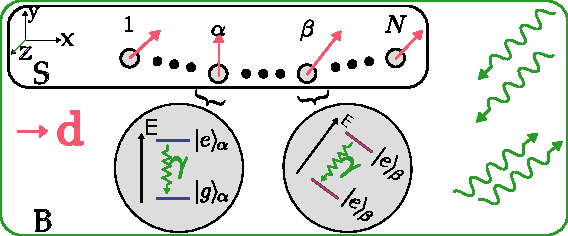
\includegraphics[width=0.6\textwidth]{N_atoms_w_dipoles}
    \caption{System S of $ N $ identical atoms, coupled to an electromagnetic bath B.
    Each carries one classical dipole-vector.
    It corresponds to the transition from the excited state $ \vert e \rangle_\alpha $ to the ground state $ \vert g \rangle_\alpha $,
    and points from the center of negative charge to the center of positive charge in the spatial distribution of the states.
    Each atom independently is subject to spontanious emission with rate $ \gamma $.}
    \label{fig:dipoles}
\end{figure}

\noindent
For the system $ \text{S} $ the quantum optical Linblad master equation
contains jump operators $\hat{L}_k$
responsible for the collective photon emission and a Hamiltonian

\begin{equation} \label{eq:Dipole_Dipole_interaction}
\hat{H}_{\text{dd}} = \hbar \sum_{\alpha, \beta} V_{\alpha\beta} \hat{\sigma}_{\alpha}^{\dagger} \hat{\sigma}_{\beta},
\end{equation}

\noindent
that represents the unitary exchange of a photon between two emitters, %(flip-flop)
%This coupling of two atoms occurs with the rate $ V_{\alpha\beta} $.
%-> not true?
with a $N \times N$ dipole-dipole interaction matrix  \(V\).
In this expression $ \hat{\sigma}_{\alpha} $ represents the lowering operators for the $\alpha$-th atom
while every other atom remains unchanged

\begin{equation}
    \hat{\sigma}_\alpha = |g_\alpha\rangle\langle e_\alpha| \equiv 1 \otimes \cdots \otimes 1 \otimes |g\rangle_\alpha \langle e|_\alpha \otimes 1 \cdots \otimes 1.
\end{equation}

\noindent
The diagonal elements of \(V\) correspond to self-interactions
like the so-called Lamb shift (caused by vacuum fluctuations of the radiation field)
which slightly alters the energy levels of the atoms.
These effects are small compared to the collective behaviors like the dipole-dipole interactions,
as this work focuses on a low-energy regime.
Therefore, they are neglected by setting \(V_{\alpha \alpha} = 0\) for all \(\alpha\) \cite{Asenjo-Garcia2017, Ma2024}.
%This interaction makes the atoms “distinguishable” from each other and reduces the high correlation of the pure symmetrical states, leading to the effect of subradiance in this system \cite{GROSS1982301}.
%I dont understand this sentences above

\noindent
The single atom lowering operators are connected to the collective jump operators via a superposition

\begin{equation}
    \hat{L}_k = \sum_{\alpha=1}^{N} c_{k, \alpha} \hat{\sigma}_{\alpha},
    \quad \text{where} \quad
    \sum_{\alpha=1}^{N} c_{k, \alpha}^* c_{\mu, \alpha} = \delta_{k\mu}
    \quad \text{and} \quad
    \sum_{k=1}^{N} \Gamma_k |c_{k,\alpha}|^2 = \Gamma_0,
\end{equation}

\noindent
where $\delta_{k\mu}$ is the Kronecker delta and $c_{k,\alpha}$ the spatial profile of the $k$-th jump operator \cite{Masson2022}.

\noindent

\noindent
As mentioned earlier,
the master equation (the extension of Eq. \eqref{eq:1atomME} to $N$ atoms)
can be rewritten with the use of a matrix $\Gamma$ as \cite{Clemens2003}

\begin{equation}\label{eq:QuantumOptical_ME}
\frac{d\hat{\rho}}{dt} = -\frac{i}{\hbar} [\hat{H}_{\text{dd}}, \hat{\rho}] + \sum_{\alpha,\beta} \Gamma_{\alpha\beta} \left( \hat{\sigma}_{\beta} \hat{\rho} \hat{\sigma}_{\alpha}^\dagger - \frac{1}{2} \left\{ \hat{\sigma}_{\alpha}^\dagger \hat{\sigma}_{\beta}, \hat{\rho} \right\} \right) ,
\end{equation}

\noindent
where $ \Gamma_{\alpha\beta} $ describe the dissipative couplings between the atoms and represent the spontaneous emission of the system.

\noindent
Each operator in the master equation acts on states in the Hilbert space of dimension $2^N$.
When calculating the evolution of a photonic excitation,
a set of equations with as many equations as the dimension of the density matrix has to be solved.
The exponential scaling with the atom number leads to difficulties
for large systems (e.g. $  N > 20 $).
Because of this, for bigger systems, techniques for dimension
reduction are necessary.
The next section brings Eq.
\eqref{eq:QuantumOptical_ME}
into a tangible form via an effective Hamiltonian in order to then apply such a reduction.


%-----------------------------------
%	SUBSECTION 1
%-----------------------------------
\subsection{Effective Hamiltonian}\label{subsec:H_eff}
Each commutator and anti-commutator can be expanded, and Eq. \eqref{eq:Dipole_Dipole_interaction} inserted to obtain
\begin{equation}
\begin{aligned}
\frac{d\hat{\rho}}{dt} &= -i \sum_{\alpha , \beta} V_{\alpha\beta} \left[-  \hat{\sigma}_{\alpha}^{\dagger} \hat{\sigma}_{\beta} \hat{\rho} +  \hat{\rho} \hat{\sigma}_{\alpha}^{\dagger} \hat{\sigma}_{\beta} \right]
 + \sum_{\alpha,\beta} \frac{\Gamma_{\alpha\beta}}{2} \left( 2 \hat{\sigma}_{\beta} \hat{\rho} \hat{\sigma}_{\alpha}^\dagger - \hat{\sigma}_{\alpha}^\dagger \hat{\sigma}_{\beta} \hat{\rho} - \hat{\rho} \hat{\sigma}_{\alpha}^\dagger \hat{\sigma}_{\beta} \right)\\
&= -i \left[ \sum_{\alpha , \beta} \left( - V_{\alpha\beta} \hat{\sigma}_{\alpha}^{\dagger} \hat{\sigma}_{\beta} - \frac{i}{2} \Gamma_{\alpha\beta} \hat{\sigma}_{\alpha}^\dagger \hat{\sigma}_{\beta} \right) \hat{\rho} \right. \\
&\quad \quad \quad + \left. \hat{\rho} \sum_{\alpha , \beta} \left( V_{\alpha\beta}  \hat{\sigma}_{\alpha}^{\dagger} \hat{\sigma}_{\beta} - \frac{i}{2} \Gamma_{\alpha\beta} \hat{\sigma}_{\alpha}^\dagger \hat{\sigma}_{\beta} \right) \right] \\
&\hspace{0.48cm}   + \sum_{\alpha,\beta} \Gamma_{\alpha\beta} \hat{\sigma}_{\beta} \hat{\rho} \hat{\sigma}_{\alpha}^\dagger .
\end{aligned}
\end{equation}

\noindent
A non-Hermitian effective Hamiltonian $ \hat{\mathcal{H}}_{\text{eff}} $ can be introduced as
\begin{equation} \label{eq:H_eff}
    \hat{\mathcal{H}}_{\text{eff}} = \sum_{\alpha, \beta} \left(- V_{\alpha\beta} - \frac{i}{2} \Gamma_{\alpha\beta} \right)\hat{\sigma}_{\alpha}^{\dagger} \hat{\sigma}_{\beta}.
\end{equation}

\noindent
Now the master equation describing the atomic system simplifies to
\begin{equation}
    \frac{d\hat{\rho}}{dt} = - i \left( \hat{\mathcal{H}}_{\text{eff}} \hat{\rho} - \hat{\rho} \hat{\mathcal{H}}_{\text{eff}}^\dagger \right) + \mathcal{D}(\hat{\rho}),
\end{equation}

\noindent
with
\begin{equation}
\mathcal{D}(\hat{\rho}) = \sum_{\alpha,\beta} \Gamma_{\alpha\beta} \hat{\sigma}_{\beta} \hat{\rho} \hat{\sigma}_{\alpha}^\dagger,
\end{equation}
describing the emission of a photon.
In the following section, a restricted subspace will be found,
where the computations for calculating an evolution are significantly reduced to order $ \mathcal{O}(N) $.



%----------------------------------------------------------------------------------------
%	SUBSECTION 2
%----------------------------------------------------------------------------------------
\subsection{Dynamics in the single excitation subspace} \label{sec:Single_Excitation}
%\cite{BRANDES2005315}:Single modes
The system is initially restricted to a superposition of single excitations
$\vert e_{\alpha} \rangle \equiv \vert g\rangle_1 \otimes \cdots \otimes \vert e\rangle_\alpha \otimes \cdots \otimes \vert g\rangle_N$, for all $\alpha = 1, \ldots, N$.
This means that exactly one, unknown atom is excited.
As mentioned above, the effective Hamiltonian $\hat{\mathcal{H}}_{\text{eff}}$ is responsible for the evolution of the initial state.
Due to dissipation into the environment, the number of excitations can only decrease to zero.
Consequently, the dynamics can be described within a truncated Hilbert space spanned by the many-body ground state
$\vert G\rangle \equiv \vert g\rangle_1 \otimes \vert g\rangle_2 \otimes \cdots \otimes \vert g\rangle_N$
and the single-excitation states $\vert e_{\alpha} \rangle$ \cite{Bienaime2012}.
The dynamics in the single-excitation subspace decouple from the rest \cite{Needham2019}.
This can be seen by inserting the ansatz for the density matrix

\begin{equation}
    \hat{\rho} = \begin{pmatrix}
        \rho_{\text{GG}} & \bm{\rho}_{\text{Ge}} \\
        \bm{\rho}_{\text{eG}} & \rho_{\text{ee}}
        \end{pmatrix} \text{,}
\end{equation}

\noindent
where $\rho_{\text{GG}} = \langle G \vert \hat{\rho} \vert G \rangle$,
$\bm{\rho}_{\text{Ge}} = \langle G \vert \hat{\rho} \vert \bm{e} \rangle$,
$\bm{\rho}_{\text{eG}} = \langle \bm{e} \vert \hat{\rho} \vert G \rangle$, and
$\rho_{\text{ee}} = \langle \bm{e} \vert \hat{\rho} \vert \bm{e} \rangle$,
with $\vert \bm{e} \rangle$ being a column vector
containing all single-excitation states $\vert e_{\alpha} \rangle$.
Inserting this into Eq.~\eqref{eq:ME_in_Linblad_form}, the matrix equation

\begin{equation}
    \frac{d}{dt} \rho_{\text{ee}} = -i \left[ H_{\text{eff}} \rho_{\text{ee}} - \rho_{\text{ee}} H_{\text{eff}}^\dagger \right]
\end{equation}

\noindent
is obtained with a new effective Hamiltonian

\begin{equation} \label{eq:reduces_H_eff}
    H_{\text{eff}} = V - \frac{i}{2} \Gamma,
\end{equation}

\noindent
where $ V $ and $ \Gamma $ are the matrices
with entries $V_{\alpha \beta}$ and $\Gamma_{\alpha \beta}$ respectively.
They are of size $N \times N $, which significantly reduces the computational power needed to calculate the time evolution of a state.

\noindent
In this subspace, the atoms can equivalently be treated like classical dipoles \cite{AsenjoGarcia2017},
which justifies the usage of $\mathbf{d}$ in \autoref{fig:dipoles}.
The dipole vector of an atom is defined by the matrix elements of the quantum mechanical dipole operator $\hat{\mathbf{d}} = q \mathbf{\hat{r}} $. %\cite{Asenjo-Garcia2017}.
The dipole vector corresponding to the transition of the $\alpha$-th atom is $\mathbf{d}_\alpha = _{\alpha}\langle g \vert \hat{\mathbf{d}}_\alpha \vert  e \rangle_{\alpha}$.


\noindent
The coefficients $V_{\alpha \beta}$ and $\Gamma_{\alpha \beta}$ can be calculated by the real and imaginary part of
$\mathbf{G}$ (which is analytically given by Eq. \eqref{eq:Green_vacc}) \cite{Asenjo-Garcia2017}

\begin{equation}\label{eq:V_matrix}
V_{\alpha \beta} = \frac{\omega_\alpha^2}{\hbar \epsilon_0 c^2}\mathbf{d}_\alpha^T \mathrm{Re}[\mathbf{G}(\mathbf{r}_\alpha, \mathbf{r}_\beta, \omega_\alpha)] \mathbf{d}_\beta
\end{equation}

\noindent
and

\begin{equation}\label{eq:Gamma_matrix}
\Gamma_{\alpha \beta} = \frac{2 \omega_\alpha^2}{\hbar \epsilon_0 c^2}\mathbf{d}_\alpha^T \mathrm{Im}[\mathbf{G}(\mathbf{r}_\alpha, \mathbf{r}_\beta, \omega_\alpha)] \mathbf{d}_\beta.
\end{equation}

\noindent
The diagonal elements of \(\Gamma\) correspond to the single-atom decay rate and can now be calculated  \(\Gamma_{\alpha \alpha} = \frac{2 \omega_\alpha^2}{\hbar \epsilon_0 c^2} \vert \mathbf{d}_{\alpha} \vert^2 \equiv \gamma\).
When the distance between atoms is comparable to the transition wavelength,
\(d \approx \lambda_0\) collective sub- and superradiance arises
(see \autoref{sec:Coherent_Dissipation}).
The off-diagonal elements satisfy \(0 \leq \Gamma_{\alpha \beta} \leq \gamma\), approaching \(\gamma\) or zero when the interatomic distance is small or large compared to the wavelength, respectively.
%In total, this matrix has positive eigenvalues.

\noindent
An effective equation of motion in the single excitation subspace was found.
With the explicit formulas for $ V $ and $ \Gamma $, that depend on the atomic transition, which is fixed, and the topology
(how the atoms are arranged and how the dipoles are orientated),
the evolution of an initial excitation on the system can be calculated.
The next section presents a measure for how good the atoms retain the excitation that is also a great tool to visualize the evolution.



%----------------------------------------------------------------------------------------
%	SUBSECTION 3
%----------------------------------------------------------------------------------------
\subsection{Survival probability}

\noindent
For the system of \( N \) atoms and for simplicity, the initial state is restricted to be a pure state, where \( \rho_{ee}(0) = \vert \psi(0) \rangle \langle \psi(0) \vert \).
Such an initial state evolves under the non-Hermitian Hamiltonian \( H_{\text{eff}} \) and stays pure.
% why can we use normal QM evolution here?? \todo
Because the Hamiltonian is time-independent, the state $\vert  \psi(t) \rangle$ can be expressed as

\begin{align} \label{eq:Phase_Decay}
\vert  \psi(t) \rangle = \exp{\left(-\frac{i}{\hbar} H_{\text{eff}} t\right)} \vert  \psi(0) \rangle =
\underbrace{\exp(-i V t)}_{\text{Phase}} \,
\underbrace{\exp(-\frac{\Gamma}{2} t)}_{\text{Decay}} \,
\vert  \psi(0) \rangle \text{.}
\end{align}

\noindent
Here the Baker–Campbell–Hausdorff formula was used to separate the operators.
The survival probability, describing the probability for not emitting a photon into the radiation field,
is given by the norm of the state described by Eq. \eqref{eq:Phase_Decay} and can be written as

\begin{equation}
    P_{\text{sur}}(t) = \vert \vert  \psi(t) \rangle \vert^2 = \sum_{\alpha=1}^{N} \vert c_{\alpha}(t) \vert^2 \text{.}
\end{equation}

\noindent
where \( \vert c_{\alpha}(t) \vert^2 \) represents the probability amplitude of the \(\alpha\)-th atom being excited at time \( t \).

\noindent
On the one hand, the matrix $ V $ contributes a phase in the evolution.
On the other hand, the equation for the density matrix is trace-preserving ($\text{Tr}[\rho] = 1$) and
$ \Gamma $ can again be connected to the dissipative dynamics, reducing the survival probability over time.
The population of the ground state $ \rho_{GG} $ increases over time.

\noindent
Thus, the survival probability quantifies how the system retains its excitation as it evolves.
It is also a great tool to visualize the evolution of a photonic excitation on the atomic system and will be used in \autoref{Chapter4}.




%----------------------------------------------------------------------------------------
%	SECTION 3
%----------------------------------------------------------------------------------------
\section{Reciprocal space} \label{sec:K-space}
The reciprocal space emerges as an important tool in the analysis of periodic systems.
Here the phase velocity can be designed for an effective excitation transport, also to be used in \autoref{Chapter4}.


\noindent
The simplest lattice is an infinitely long one-dimensional chain with sites $ \mathbf{r}_\alpha$,
and exhibits translational symmetry by any lattice vector $\mathbf{R}$.
This work focuses on the transport of an excitation on a chain of atoms.
The chain can be seen as the system S of \autoref{sec:Adapt_to_System}.
When all dipoles are aligned, the components of the Green's tensor (Eq. \eqref{eq:Green_vacc}) are translationally invariant.
Then, Blochs theorem \cite{Bloch1929} allows the diagonalization of $ \mathbf{G} $ via a Fourier transformation.
This way the eigenfunctions of $ \mathbf{G} $ can be expressed as plane waves

\begin{equation}
\vert k_i \rangle = \frac{1}{\sqrt{N}} \sum_{\alpha =1 }^{N} \langle e_\alpha \vert k_i \rangle  \vert e_\alpha \rangle
= \frac{1}{\sqrt{N}} \sum_{\alpha =1 }^{N} e^{i k_i |\mathbf{r}_{\alpha}|} \vert e_\alpha \rangle \text{.}
\end{equation}

\noindent
The Fourier transformation can be written in matrix form as

\begin{equation} \label{eq:FT}
T \equiv \left[\vert k_1 \rangle \dots \vert k_i \rangle \dots \vert k_N \rangle \right] \text{,}
\end{equation}

\noindent
and can be used to perform a change of basis between real- and reciprocal/($k$)-space.
Here $\vert k_i \rangle$ denotes the i-th eigenstate in $k$-space.
The Green's tensor is diagonal in this basis with eigenvalue $ G_{k_i} $.
One can directly connect a pseudo momentum $ k $ in the first Brillouin zone $ k \in [-\pi/d,\pi/d] \subset \mathbb{R} $ with each eigenvalue.
This reducibility comes from the fact that each state $ \vert k \rangle $ is unique up to a constant reciprocal lattice vector $\vert\mathbf{K}\vert = 2 \pi / \text{d}$.
Here $d$ is the distance of two neighboring atoms.
The real and imaginary part of the eigenvalues is directly proportional to the eigenvalues $ V_k $ and $ \Gamma_k $ respectively
(see Eqs.~\eqref{eq:V_matrix} and \eqref{eq:Gamma_matrix}).
Thus, the effective Hamiltonian Eq. \eqref{eq:reduces_H_eff}
is diagonal in $k$-space.
This relationship reveals regions of superradiance and subradiance.
Recall that superradiant modes correspond to \(\Gamma_k > \gamma\), while subradiant modes correspond to \(\Gamma_k < \gamma\).
Notably, subradiance in free space occurs for $d \leq \lambda_0/2$, at the boundaries of the Brillouin zone, away from its center.
Asenjo-Garcia et al. \cite{AsenjoGarcia2017} showed,
that the most subradiant mode decreases with the systems size $ \Gamma_{k, \text{min}} \propto N^{-3} $,
motivating the usage of a higher atomic number in \autoref{Chapter4}.
But it should be noted
that these modes are challenging
to create experimentally due to their location in \(k\)-space as well as their complicated phase pattern \cite{Cech2023}.



%----------------------------------------------------------------------------------------
%	SUBSECTION 4
%----------------------------------------------------------------------------------------
\subsection{Group velocity} \label{subsec:Phase_vel_Control}

\noindent
With Eq. \eqref{eq:Phase_Decay}, one can argue that only the V matrix defines the spectrum of the effective Hamiltonian.
By diagonalizing \(V\), one can extract the eigenenergies \(V_k\).
The phase \( \varphi \) of the evolved state in Eq. \eqref{eq:Phase_Decay} is given by

\begin{equation}
\varphi(t) \equiv V_k t + \varphi_0
\end{equation}

\noindent
where $\varphi_0$ denotes the phase of the initial state $\vert  \psi(0) \rangle$.
The gradient of the spectrum, \(V_k\), determines the dispersion relation,
which ultimately depends on atomic positions and dipole orientations.
Without loss of generality, a wave-packet $ \vert  \psi(0) \rangle $ can be localized in $k$-space.
For instance, a Gaussian wave packet in $k$-space also remains Gaussian in real space after a Fourier transform.
By controlling the shape of the wave packet in \(k\)-space, one can manipulate the behavior of excitation on the atoms.
For a sufficiently large interval with an approximately linear spectrum,
the definition of a group velocity $ v_\text{g} $ of the wave packet is possible.
This group velocity is thus proportional to the eigenenergies

\begin{equation}
    v_\text{g} \propto \nabla \varphi \equiv \nabla V_k \cdot t.
\end{equation}

\noindent
This approach also holds as a good approximation for large but finite systems,
which can be seen in \autoref{sec:Diagonalization} of the Appendix.

\noindent
One application of this is to trap photons on specific lattice sites through a flat dispersion \cite{Cech2023}.
Another application involves initializing the wave packet in a region of \(k\)-space with an approximately linear dispersion relation.
In this scenario, the wave packet propagates with a nearly constant group velocity, avoiding dispersion during its evolution \cite{Needham2019}.
By tuning the atomic chain's structure and selecting appropriate initial conditions for the wave packet, one can effectively control the phase velocity and, consequently, the dynamics of the system.
\chapter{Presentation of the basis of this work} \label{Chapter3}
This thesis is based on the paper \cite{Startingpoint} by Botarelli.
There, a quantum router on the topology of a graph with six nodes
(see \autoref{fig:botarellis_topo}) was analyzed which will be explained in this chapter.
In the next chapter, this will be adapted to an atomic system.

\begin{figure}[!ht]
    \centering
    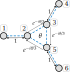
\includegraphics[width=0.5\textwidth]{Botarellis_Topo}
%    \decoRule
    \caption{The minimal graph of the quantum router in \cite{Startingpoint}.
    The circles correspond to nodes and the arrows indicate edges, the interaction between the nodes.
    Small arrows point from each node to their label (a number from 1 to 6).
    The edges with a phase point only in one direction, because the interaction is not symmetric.
    The inner loop carries weights that add up to a phase $\theta$.
    Eq. \eqref{eq:Bot_Hamilton} describes the graph intirely.}
    \label{fig:botarellis_topo}
\end{figure}

\noindent
Graphs are mathematical structures used to model pairwise relations between $N$ nodes.
In this context, nodes represent quantum objects and edges represent interactions between them.
On such a system, classical information is defined as an excitation of one of the nodes.
The node-basis trivially corresponds to the Euclidean basis
\begin{equation}
\vert i\rangle\equiv(0,\dots,\underbrace{1}_{i},\dots,0)^T\text{, for } \alpha = 1, ..., N.
\end{equation}

\noindent
indicating a classical excitation of the $i$-th node.
The quantum mechanical extension of information would be the superposition of classical excitations of nodes.
A Laplacian matrix $ L $ encodes the connectivity of a classical graph.
% Key objects are the adjacency matrix, , and degree matrix
Bottarelli's work extends the Laplacian matrix to allow for complex entries, resulting in a Hermitian Hamiltonian $ H $.
The interactions between two nodes is the complex conjugate of the reverse interaction.
The topology that was analyzed is depicted in \autoref{fig:botarellis_topo} and can be described by the $ 6 \times 6 $ matrix\footnote{The labels of the nodes 4 and 5 were switched in this definition,
    to be consistent with the definition of the system used later in this thesis.
    Such a relabeling has no effect on the physical properties.}

\begin{equation} \label{eq:Bot_Hamilton}
H
=
\begin{pmatrix}
0 & 1 & 0 & 0 & 0 & 0 \\
1 & \gamma & e^{-i \theta / 3} & 0 & e^{i \theta / 3} & 0 \\
0 & e^{i \theta / 3} & \gamma & 1 & e^{-i \theta / 3} & 0 \\
0 & 0 & 1 & 0 & 0 & 0 \\
0 & e^{-i \theta / 3} & e^{i \theta / 3} & 0 & \gamma & 1 \\
0 & 0 & 0 & 0 & 1 & 0
\end{pmatrix},
\end{equation}

\noindent
where specific edges carry a phase given by $\theta$.
The nodes of the inner triangle are connected to themselves, by a factor $ \gamma $.
The identification of the Hamiltonian $ H $
representing the interaction allows the use of quantum mechanical time evolution
to evolve an initial excitation
($\vert \psi (t = 0) \rangle = \sum_{\alpha = 1}^{6} c_\alpha(t = 0) \vert \alpha \rangle $) on the system.
The evolution breaks the time-reversal symmetry, one says it is chiral, because of the phase in the Hamiltonian.
This system-defining parameter is obtained when going along the loop in the graph \autoref{fig:botarellis_topo}.
It is the only quantum part of this analysis, enabling chirality and thus directional routing of information \cite{Ann_Springer, Shu2024}.
The result of Botarelli was that a phase-dependant directional transport of the classical state $\vert \psi_0 \rangle = \vert 1 \rangle $ is possible and robust.
This is shown in \autoref{fig:The_Basis_evolution}.
After a time $T$ a high probability can be achieved to route the initial state into one of the nodes
$ \vert 5 \rangle / \vert 6 \rangle$ while a low probability of being routed into the other nodes $\vert 6 \rangle / \vert 5 \rangle $ is guaranteed.

\begin{figure}[!ht]
    \centering
    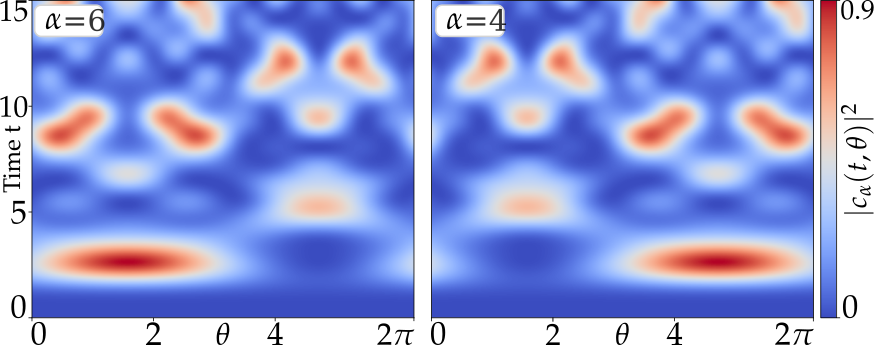
\includegraphics[width=0.8\textwidth]{The_Basis_evolution}
%    \decoRule
    \caption{The probabilities $ |c_\alpha(t) |^2 $ with $ c_1(0) = 1 $  plottet against time $t$ and the total phase $\theta$ of the loop in \autoref{fig:botarellis_topo}.}
    \label{fig:The_Basis_evolution}
\end{figure}

\noindent
The phase in the triangle is not necessary to be equally distributed along the three connections.
The evolution is only dependent on the total phase $ \theta $.
However, a symmetrical allocation makes analytical calculations manageable.

%\begin{figure}[h!]
%    \centering
%    \begin{minipage}{0.5\textwidth}
%        \begin{equation} \label{eq:Bot_Hamilton}
%            H\footnotemark
%            =
%            \begin{pmatrix}
%                0 & 1 & 0 & 0 & 0 & 0 \\
%                1 & \gamma & e^{-i \theta / 3} & 0 & e^{i \theta / 3} & 0 \\
%                0 & e^{i \theta / 3} & \gamma & 1 & e^{-i \theta / 3} & 0 \\
%                0 & 0 & 1 & 0 & 0 & 0 \\
%                0 & e^{-i \theta / 3} & e^{i \theta / 3} & 0 & \gamma & 1 \\
%                0 & 0 & 0 & 0 & 1 & 0
%            \end{pmatrix}.
%        \end{equation}
%    \end{minipage}%
%    \hfill
%    \begin{minipage}{0.45\textwidth}
%        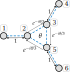
\includegraphics[width=0.8 \textwidth]{Botarellis_Topo}
%    \end{minipage}
%    \caption{The minimal graph structure used by Botarelli. The inner loop carries edge-weights of gamma. Also along the loop a phase $\theta$.}
%    \label{fig:Equation_and_Graphic}
%    \footnotetext{The indices 4 and 5 were switched in this definition to be consistent with the definition of the system used in this paper. Such a relabeling has no effect on the physical properties.}
%\end{figure}
\chapter{Adaptation of Botarellis work to atoms} \label{Chapter4}

\noindent
From the start, it is clear that directional routing as discussed in \autoref{Chapter3} is not possible with atoms.
The open system dynamics lead to an effective Hamiltonian in Eq. \eqref{eq:reduces_H_eff} which is non-Hermitian.
Thus, unlike the system in Chapter 3, a setup with $N$ atoms offers no chirality.
To qualitatively see what issues come up,
the methods from Botarelli's work are still applied to a system of six atoms in this chapter.
Then, a modified approach is developed to address these issues and later extended to $N$ atoms.


%----------------------------------------------------------------------------------------
%	SECTION 1
%----------------------------------------------------------------------------------------
\section{Challenges} \label{sec:challenges}
Botarelli's topology only has edges between adjacent nodes.
In contrast, the atomic system is much more complex, as interactions between all atoms need to be considered.
Instead of six connections, the configuration with atoms exhibits $21$ links.
The approach of reducing the fully connected case by considering only nearest-neighbor interactions fails.
This can lead to negative eigenvalues of the $ \Gamma $ matrix,
resulting in an unphysical increase in the survival probability (see Eq. \eqref{eq:Phase_Decay}).
Consequently, the exact quantum router proposed in Botarelli's paper cannot be adapted to an atomic system.

\noindent
A similar phase as in \autoref{fig:botarellis_topo} can be defined and effectively influenced by the atomic separation and the orientation of their dipoles.
This will be shown now.

%-----------------------------------
%	SUBSECTION 1
%-----------------------------------
\subsection{Phase control} \label{subsec:Phase_control}
Generally the entries of the effective Hamiltonian $ H_{\text{eff}} $ from Eq. \eqref{eq:reduces_H_eff} are complex numbers,
which connect two atoms with indices $\alpha \text{ and } \beta$.
A phase $\Phi_{\alpha\beta}$ of the complex number,
defined as the polar angle in the complex plane,
can be extracted analytically as

\begin{equation} \label{eq:phase_of_H_ab}% \todo[+- pi/2 oder so]
    \Phi_{\alpha\beta}(\mathbf{r}_\alpha, \mathbf{r}_\beta, \mathbf{d}_\alpha, \mathbf{d}_\beta) \equiv \arctan\left( \frac{\Gamma_{\alpha\beta}}{2V_{\alpha\beta}} \right),
\end{equation}

\noindent
where $ \mathbf{r}_{\alpha,\beta} $ are the position vectors of the two atoms and $ \mathbf{d}_{\alpha,\beta} $ their dipoles
as defined in \autoref{sec:Adapt_to_System}.
The dependence of these four parameters is clear from the definitions of $ V $ and $ \Gamma $ in \autoref{sec:Single_Excitation}.
At first, the minimal example, a system of two atoms is considered.
\autoref{fig:N_2_Matrixemtry(r)} illustrates the off-diagonal element in $ V $ and $ \Gamma $ for different dipole orientations and interatomic distances.
Generally, dipoles with arbitrary orientations are permitted, which is shown on the right side of the figure.

\begin{figure}[!ht]
    \centering
    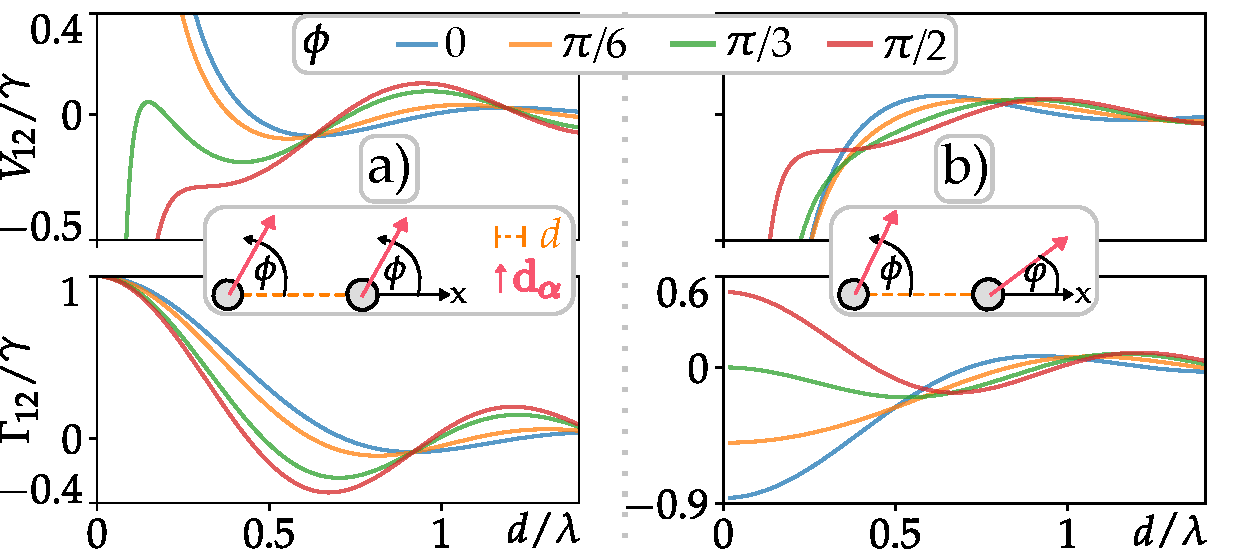
\includegraphics[width=0.8\textwidth]{2_atoms_Matrix_elems_combined(r)}
%    \decoRule
    \caption{The matrix element $ V_{12} $ and $ \Gamma_{12} $ represents the interaction strength between two atoms (dipole-dipole aswell as dissipation).
             They are plotted in units of $ \gamma $ against their separation $ d $ for different angles $ \phi $, which is measured with respect to the $x$-axis.
             \textbf{a)} Both dipoles are aligned.
             \textbf{b)} One dipole is fixed at $ \varphi = 5\pi/6 $ and one is varied.}
    \label{fig:N_2_Matrixemtry(r)}
\end{figure}

\noindent
To get closer to the desired setup, the number of atoms is now increased to $N = 3$.
The dipoles are assumed to lie within the plane defined by the resulting atomic triangle.
%as this is a physical approach.
This triangular configuration can be compared to the loop in \autoref{fig:botarellis_topo}.
The total phase \( \theta \)

\begin{equation}
    \theta \equiv \theta (\mathbf{r}_1, \mathbf{r}_2, \mathbf{r}_3, \mathbf{d}_1, \mathbf{d}_2, \mathbf{d}_3) \equiv  \Phi_{12} + \Phi_{23} + \Phi_{31},
\end{equation}

\noindent
can be defined, which represents the phase accumulated around the triangle.
To investigate the significance of $ \theta $, one can sum the three phases of Eq. \eqref{eq:phase_of_H_ab}
clockwise.
It turns out that when summing anticlockwise, the phase is the same, unlike in \autoref{Chapter3} (where the sign of $ \theta $ changes).
This is due to the Hamiltonian of the system being symmetric (and not Hermitian as in the work of Botarelli).
In addition,
it becomes evident, that different atomic separations and dipole orientations can add to the same phase $ \theta $.
This is shown in detail in \autoref{sec:No_direcionality} of the Appendix.

\noindent
In summary, it can be stated that, in contrast to the work of Botarelli, the phase $ \theta $ is not anymore the system-defining parameter.
The system of atoms is primarily characterised by the atomic separations and dipole orientations.

\noindent
While $ \theta $ is built up of these parameters, it does not provide the uniqueness of the system.
Different configurations add to the same $ \theta $,
and still result in distinct evolutions of the same excitation, contrary to \autoref{fig:The_Basis_evolution}.
In the following sections,
a condition will be introduced to still induce directional routing on the atomic system without the use of this phase.


%----------------------------------------------------------------------------------------
%	SECTION 2
%----------------------------------------------------------------------------------------
\section{Conditions for directional routing}\label{sec:solutions}
As described directional routing with atoms is not inherently possible by varying $\theta$.
However, one can achieve a controlled evolution by choosing specific dipole orientations and interatomic distances.
Without loss of generality, this work focuses on routing an excitation from the left into the upper arm.
Due to the system's symmetry along the $x$-axis, the results can be mirrored to achieve routing toward the lower arm as well.
To route an excitation into the upper arm, the matrix entries should satisfy the conditions

\begin{equation} \label{eq:Conditions}
\frac{V_{13}}{V_{12}} \ll 1 \quad \text{and} \quad \frac{V_{23}}{V_{12}} \ll 1 \text{.}
\end{equation}

\noindent
Here, the indices 1, 2 and 3 represent the atom of the triangle.
As described in \autoref{fig:N_2_Matrixemtry(r)}, changing the dipole orientation of different atoms modifies the elements $V_{\alpha \beta}$.
This modification can be helpful in meeting the conditions specified in Eq. \eqref{eq:Conditions}.
To explore this further, three topologies are investigated, illustrated in the upper part of \autoref{fig:Three_Topologies_and_optimization}.
%%Each of the systems will later be extended to configurations with $N > 6$ atoms.
For bigger systems,
additional atoms $N \geq 6$ are placed outside the triangle on extended lines between the center of the triangle
and the edge atoms.
The distances of these "outer" atoms are fixed at $d_\text{ext}$,
while the inner distance $d$ is varied.

\begin{figure}
    \centering
    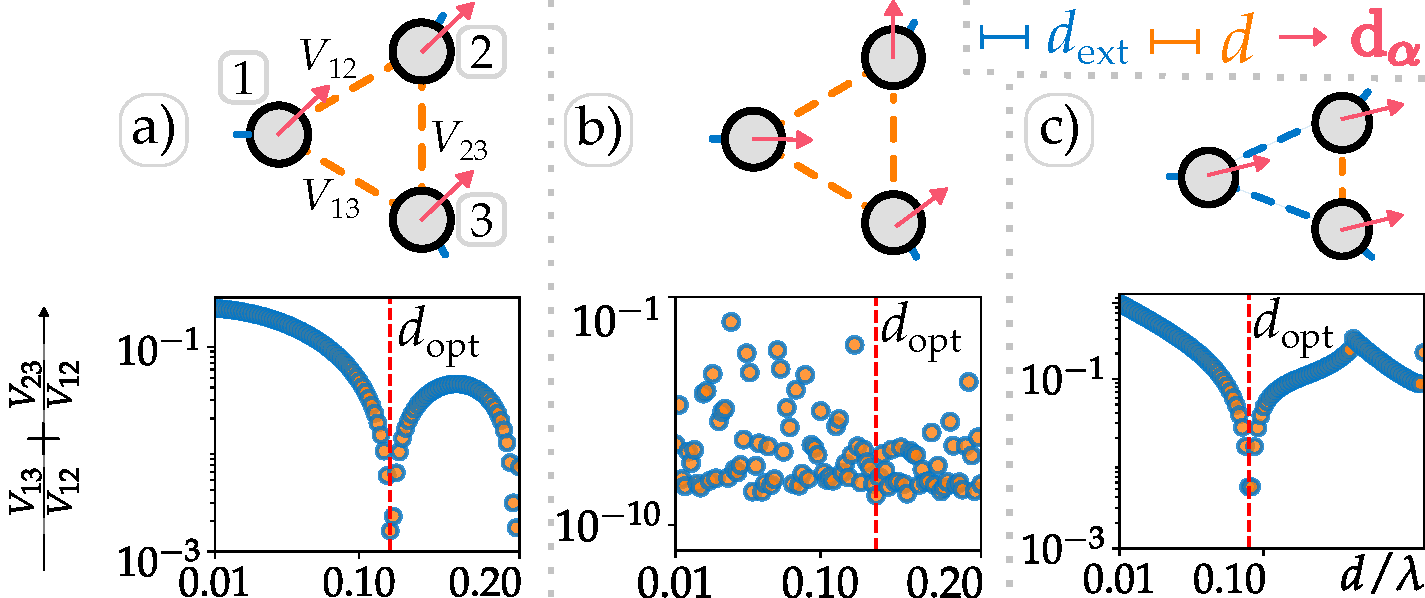
\includegraphics[width=0.8\textwidth]{Ratios_for2_Solutions}
%    \decoRule
    \caption{\textbf{a)} Equilateral triangle with aligned dipoles.
%    The dipoles are again measured with respect to the x-axis.
    \textbf{b)} Equilateral triangle with unique dipole orientations.
    \textbf{c)} Isosceles triangle, where one inner distance is changed and the dipoles are aligned.
    The dipole-dipole coupling strength $ V_{\alpha \beta} $ between each atom is indicated along the connection of two atoms.
    Each system will be investigated with $ N > 3 $ later, indicated by the small blue connections at each atom.
    \textbf{Conditions: }
    For each distance $ d $, there exists a set of dipole orientations,
        such that the ratios (Eq.
        \ref{eq:Conditions}) are minimal.
    % (measured with respect to the x-axis)
    The sum of these ratios is plotted with a logarithmic scaling against $ d $ in units of $\lambda$.
    Additionally, each topology offers one distance $ d_{\text{opt}} $, where the sum is minimal.
    An external distance of $ d_{\text{ext}} = 0.1 \lambda $ was used.}
    \label{fig:Three_Topologies_and_optimization}
\end{figure}

\noindent
The lower part of \autoref{fig:Three_Topologies_and_optimization} shows
that the two configurations with aligned dipoles (\textbf{a)} and \textbf{c)}) have a clear optimal distance, while
\textbf{b)} offers overall smaller values of the sum of both conditions in Eq. \eqref{eq:Conditions}.
It was separately checked that both conditions are small, and not just their sum.

\noindent
%For the Equilateral triangle, with aligned dipoles only 26\% and 66\% of the distances resulted in a setup,
%which satisfied the conditions with a threshold of \( 0.01 \).
In the completely symmetric system (\autoref{fig:Three_Topologies_and_optimization} \textbf{a)}), the optimal angle is \(\phi_{\text{opt}} = 30.04^\circ\) with an optimal distance of \(d_{\text{opt}} = 0.12\lambda\).
%When allowing unique dipoles, both conditions are satisfied 100\% of the time.
For case two (\textbf{b)}) the optimal angles are \(\phi_{\text{opt,1}} = 32.08^\circ\), \(\phi_{\text{opt,2}} = 29.63^\circ\), and \(\phi_{\text{opt,3}} = 29.12^\circ\), with an optimal distance of \(d_{\text{opt}} = 0.13\lambda\).
%When only one inner distance is varied, the conditions were only met 47\% and 55\% of the time.
For the isosceles triangle (\textbf{c)}), the optimal angle is \(\phi_{\text{opt}} = 31.69^\circ\) and the optimal distance is \(d_{\text{opt}} = 0.09\lambda\).
These values will be used in the subsequent analysis unless otherwise noted.



%-----------------------------------
%	SECTION 3
%-----------------------------------
\section{Implementation of Botarelli's system with six atoms}\label{subsec:botarellis_system}
With the optimal configurations identified,
the topology
proposed in Botarelli's paper \cite{Startingpoint} can be implemented with six atoms.
Using the just determined angles in the case of an equilateral triangle with aligned dipoles, the dipole of atom 2 is oriented directly towards atom 3.
This arrangement is visualized in \autoref{fig:EVO_System_with_atoms} \textbf{a)}.

\begin{figure}[!ht]
    \centering
    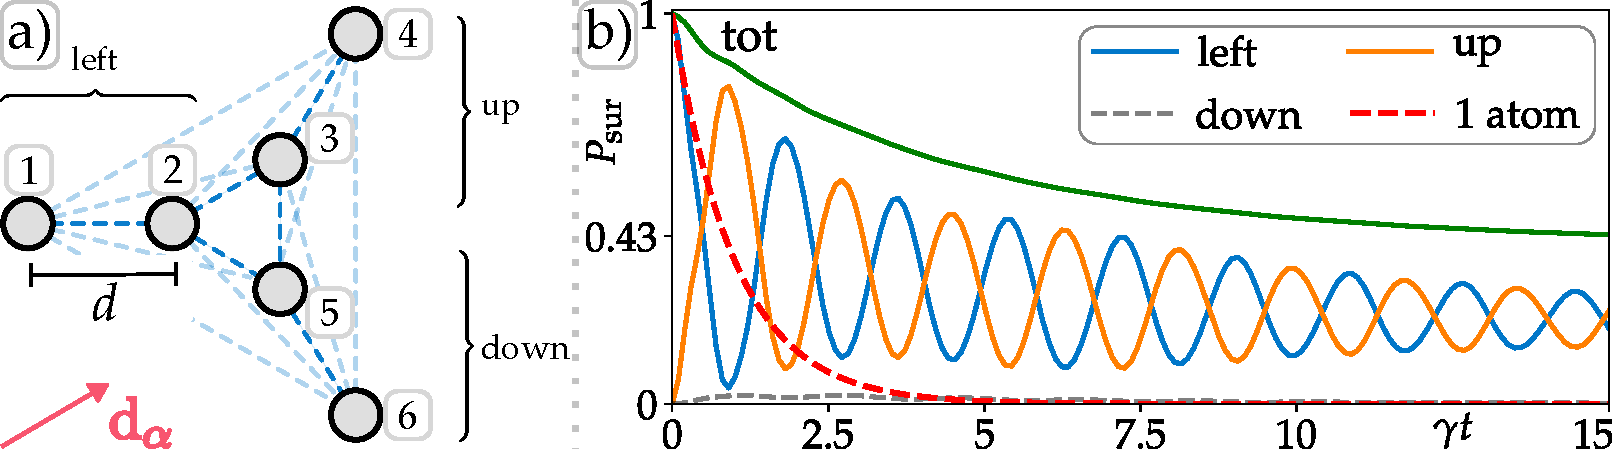
\includegraphics[width=1.0\textwidth]{System_with_atoms}
%    \decoRule
    \caption{\textbf{a)} A fully connected system of $N = 6$ atoms,
        which is maximally symmetric, mimicking the topology in \autoref{fig:botarellis_topo}.
    The dipole-dipole coupling strength $ V_{\alpha \beta} $ between each atom is indicated along the connection of two atoms.
    The opacity of a connection represents its strength, that depends on the distance between two atoms.
    The inner triangle is equilateral.
    All dipoles are  aligned indicated by $d_\alpha$.
    The system is initially in a superposition of atom 1 and 2 being excited.
    The state can mathematically be described by
    $ \vert \psi_x(0)\rangle =  \frac{1}{\sqrt{2}}\left[e^{i \varphi}, -e^{i \varphi}, 0, 0, 0, 0\right] \text{, with } \varphi \approx 1.3 $.\\ %2784
    \textbf{b)} Probability of finding the photonic excitation plotted against $ \gamma ^{-1}$.
    The total (\textbf{"tot"}) survival probability is displayed in green, while \textbf{"left"}
    means the probability of being on atoms (1,2), \textbf{"up"} refers to atoms (3,4), and
    \textbf{"down"} corresponds to atoms (5,6).
    As a reference, the red dashed line shows the single atomic behavior.}
    \label{fig:EVO_System_with_atoms}
\end{figure}

\noindent
Part \textbf{b)} shows the evolution of an initial state on the left arm.
The probability of finding the photon oscillates between the atoms (1,2) and (3,4).
The probability of being on atoms (5,6) is close to zero for all times.
\noindent
The lifetime of the photon being on the system is enhanced such that after $ T = 15 /\gamma $, the survival probability is $ 0.43$.
This can further be increased by using even more ($ N > 6 $) atoms \cite{AsenjoGarcia2017}.
This is why an initial state with a large number of atoms will now be defined.



%----------------------------------------------------------------------------------------
%	SUBSECTION 3
%----------------------------------------------------------------------------------------
\section{System definition with \texorpdfstring{$N > 6$}{N > 6}} \label{sec:Sys_def_N_bigger_6}
As discussed in section \ref{subsec:Phase_vel_Control},
the protocol for a given topology of $ N $ atoms in a specific arrangement with given dipole orientations is as follows.
First, the spectrum of the system is analyzed\footnote{The Hamiltonian of an infinite system can exactly be diagonalized with a Fourier transformation (FT).
For a finite systems, the diagonalization via a FT still holds only as an approximation (see \autoref{sec:Diagonalization} in the Appendix).
But, as discussed in \autoref{sec:K-space}, it is still useful to operate in quasi-momentum space.
}.

\noindent
In $k$-space, a Gaussian wave packet
\begin{equation}
    \vert \psi_k(t = 0) \rangle = (\sqrt{2 \pi}\sigma_k)^{-1/2} \sum_{i=1}^{N} e^{-(k-k_\text{s})^2/(4 \sigma_k^2)} \vert k_i \rangle
\end{equation}

\noindent
is initialized on a subradiant region ($\Gamma_k < 1$) with an approximately constant group velocity.
This wave packet has a peak at \( k_\text{s} \) with a width given by \( \sigma_k \).
The states $ \vert k_i \rangle $ are the $ N $ basis modes defined in \autoref{sec:K-space}.
%A phase multiplication is then applied to determine the center of the wave packet in real space.
%%e^{-i (\alpha - \nu)d_{\text{ext}}}
The state in real space can be obtained by applying the inverse Fourier transform (see Eq. \eqref{eq:FT}) to the state in $k$-space.
This resulting state maintains a Gaussian shape\footnote{Note that this relation strictly holds for an infinitely large system.
For finite systems, it should be treated with caution.
However, again, sufficiently large systems are considered here, so this relation can be used as a good approximation.} and is expressed as:

\begin{equation} \label{eq:Initial_state}
\vert \psi_x(t = 0) \rangle = \sqrt{\frac{\sigma_k}{\sqrt{2 \pi}}} \sum_{\alpha=1}^{N} e^{-i k_\text{s} \overbrace{(\alpha - \nu)d_{\text{ext}}}^{\mathbf{r}_{\alpha-\nu}}} e^{-(\alpha - \nu)^2 d_{\text{ext}}^2\sigma_k^2} \vert e_\alpha \rangle \equiv \sum_{\alpha=1}^{N} c_{\alpha}(0) \vert e_\alpha \rangle.
\end{equation}

\noindent
In this expression, \( \nu \) represents the atom index where the Gaussian has its peak.
The parameter \( d_\text{ext} \) denotes the atomic separation in the chain and
\( \vert e_\alpha \rangle \) (a real-space basis state) refers to the \( \alpha \)-th atom being excited.

%----------------------------------------------------------------------------------------
%	SUBSECTION 3.1
%----------------------------------------------------------------------------------------
\subsection{Transport}
The protocol for defining the initial state given by Eq. \eqref{eq:Initial_state} and its evolution is illustrated for a finite one-dimensional chain of $ N = 100 $ atoms in \autoref{fig:MOM_REAL_SPACE_CHAIN}.
\begin{figure}
    \centering
    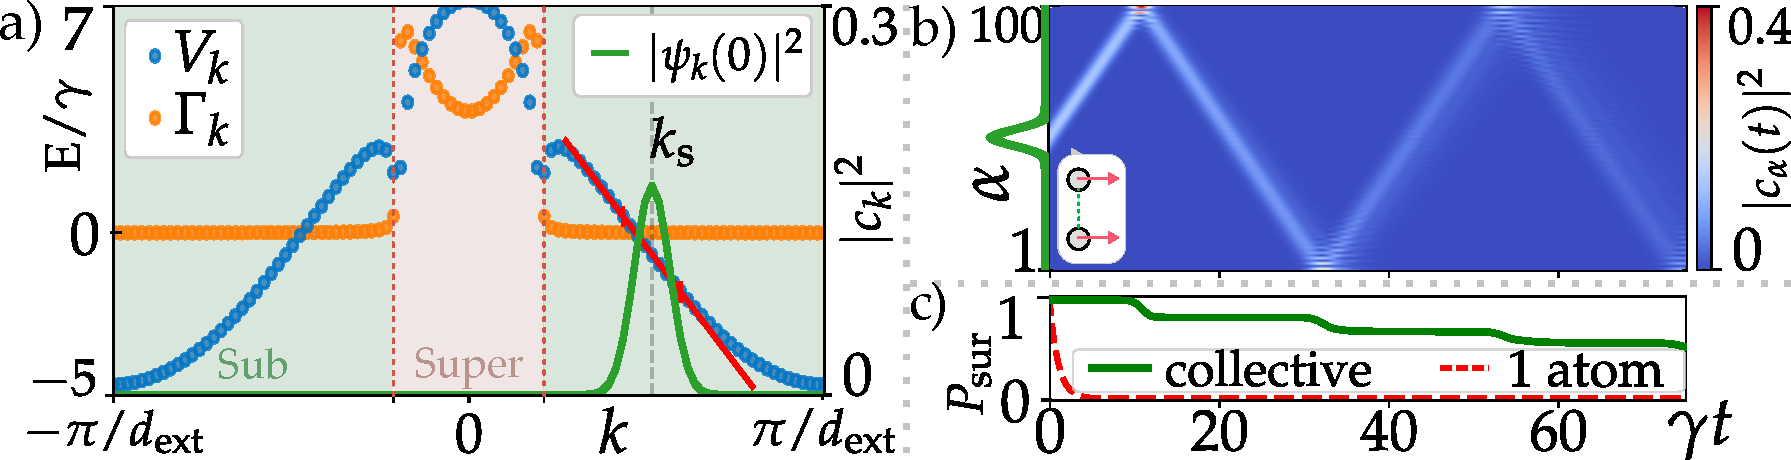
\includegraphics[width=1.0\textwidth]{CHAIN_MOM_EVO}
%    \decoRule
    \caption{The dipoles are perpendicular to the chain of $N= 100$ atoms.
    \textbf{a)} Spectrum ($ V_k $), Eigen-Decay modes ($ \Gamma_k $) and norm of the wave packet $ |\psi_k(0)|^2 $ in momentum space are plotted against the pseudo momentum $k$.
    The regions of sub- and superradiance ($ \Gamma_k < 1 \text{ and } > 1$) are shaded in green and red respectively.
    Here an interatomic distance of $ d_\text{ext} = 0.1 \lambda$ was used.
    The wave packet in $k$-space has a width of $ \sigma_k = 0.05 \frac{\pi}{d_\text{ext}} $  around $ k_\text{s} \approx 0.5 \frac{\pi}{d_\text{ext}} $.
    A straight (red line) has been fitted through to modes $ V_k $ over a range $[k_\text{s} \pm 2\sigma_k]$
        indicating a linear regime in $ V_k $.
    \textbf{b)} The initial state$ \vert \psi_x(t = 0) \rangle $,
        depicted as a green line left of the color plot is evolved.
        The probability of being on the $ \alpha $-th atom against time is plotted in units of $ \gamma^{-1}$.
    \textbf{c)} The survival probability is plotted against time in units of $\gamma^{-1}$.
        The green line indicates the total, collective survival probability,
        and the dashed red line indicates the single atom decay as a reference.}
    \label{fig:MOM_REAL_SPACE_CHAIN}
\end{figure}

\noindent
The wave packet is reflected at the chain end and slightly disperses.
When this happens, the survival probability is significantly reduced.
For the evolution in the bulk, the survival probability stays approximately constant with time.

\noindent
In the topology of interest, the $ N $ atoms are arranged into three distinct chains shown in \autoref{fig:Setup_all_inner_distances}.
The left chain (left) consists of atoms numbered from 1 to \( N/3  \),
the upper chain (up) comprises atoms numbered from \(  N/3  + 1 \) to \(  2N/3  \),
and the lower chain (down) includes the remaining atoms from \( 2N/3  + 1 \) to \( N \).
For the case of unique dipoles, the atoms on the left, up and down chain all have their own dipole angle $ \phi_{\text{opt,1,2,3}} $ respectively.
Within the chain, they are aligned.
The wave packet will only be initialized on the left chain.
All coefficients $ c_\alpha: { N/3 < \alpha \leq N} $ of the state $ \vert \psi_x(t = 0) \rangle $ are set to zero.

\begin{figure}[!ht]
    \centering
    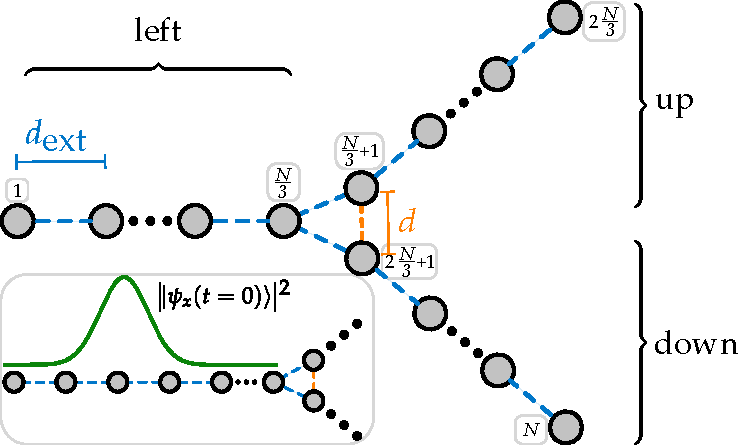
\includegraphics[width=0.75\textwidth]{system_1_inner}
    \caption{Setup for $N$ atoms with an isosceles inner triangle.
    The initial state is a Gaussian, localized near the center of the left arm as indicated by the green line.
    Full connectivity is omitted for visual clarity, although every atom interacts with every other atom.
    A similar arrangement can be made with an equilateral triangle.}
    \label{fig:Setup_all_inner_distances}
\end{figure}

\noindent
The same protocol applied to a single chain can be used here.
The shape of the spectrum depends on both the atomic distance and the dipole orientations of the left chain.
Three systems with $N$ atoms and the inner triangles according to \autoref{fig:MOM_REAL_SPACE_CHAIN} \textbf{a)},\textbf{b)} and \textbf{c)}
are used.
For cases \textbf{a)} and \textbf{b)}, the optimal inner distance is used for the external distance as well.
In contrast, with case \textbf{c)} an external distance of  $ d_\text{ext} = 0.1 \lambda $ is used.
Generally, the group velocity in the subradiant regime increases as the atomic distance in the chain decreases,
Therefore, a smaller choice of \( d_\text{ext} \) results in a faster propagation of the wave packet along the chain, allowing it to reach the inner triangle more quickly.

\noindent
When the wave packet encounters the triangle, a transmission ($T$), reflection ($R$), and a small leakage ($L$) are expected.
%, since perfect coupling cannot be achieved.
These coefficients can be defined as
\begin{equation}
    T = \frac{P_{\text{up}(t=T)}}{P_{\text{left}(t=0)}} \text{,} \quad R = \frac{P_{\text{left}(t=T)}}{P_{\text{left}(t=0)}} \quad \text{and} \quad L = \frac{P_{\text{down}(t=T)}}{P_{\text{left}(t=0)}}\text{.}
\end{equation}

\newpage
\noindent
Here, \(t=T\) represents a point in time after the routing event when each part of the original wave packet is far away from the triangle.
With this, one can measure the effectiveness of routing in the different topologies.


    %----------------------------------------------------------------------------------------
%	SECTION 4
%----------------------------------------------------------------------------------------
\newpage
\section{Routing in systems with \texorpdfstring{$N = 60$}{N = 60} atoms}
Starting from $N = 60$ a wave packet that does not couple to any superradiant modes and has a well-defined center in real space can be initialized on the system.
The evolutions for this case are shown in \autoref{fig:EVO_Topologies_N_60}.
\begin{figure}[!ht]
    \centering
    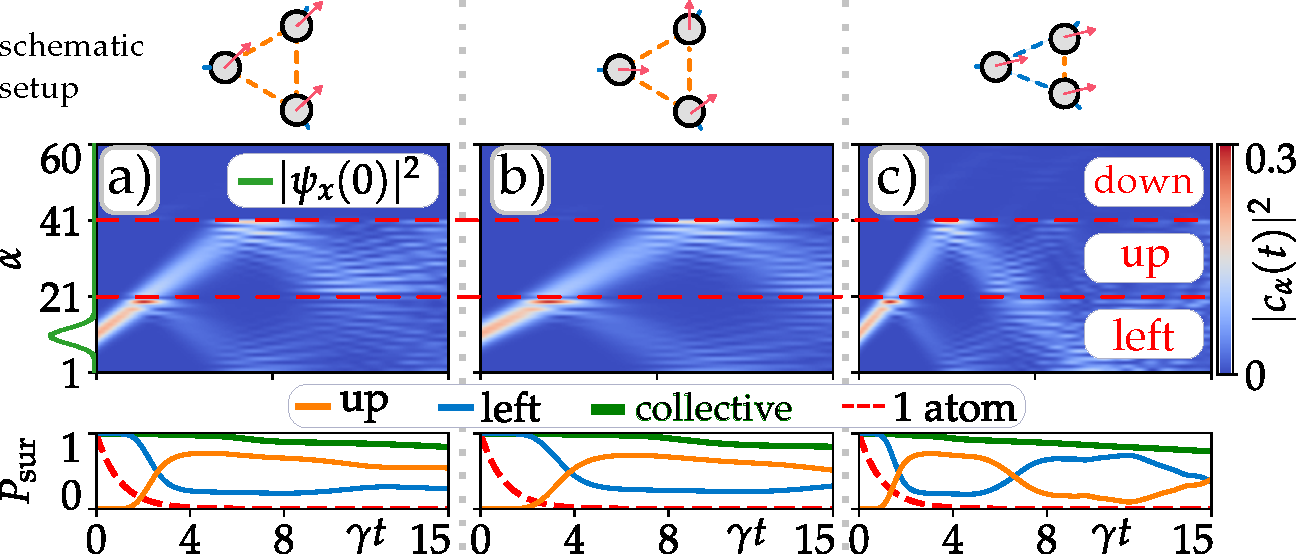
\includegraphics[width=0.8\textwidth]{Topologies_EVO_N_60}
%    \decoRule
    \caption{System with $N = 60$ atoms.
    \textbf{a)} Equilateral triangle with aligned dipoles.
    \textbf{b)} Equilateral triangle with unique dipoles.
    \textbf{c)} Isosceles triangle with aligned dipoles.
    For each system, the same initial state$ \vert \psi_x(t = 0) \rangle $,
    depicted as a green line left of the first color plot is evolved.
    The optimal setups (see section
    \ref{sec:solutions}) are used, with $\sigma_k = 0.08 \frac{\pi}{d_\text{ext}}$ and $k_\text{s} \approx 0.58 \frac{\pi}{d_\text{ext}}$.
    The probability of being on the $ \alpha $-th atom against time is plotted in units of $ \gamma^{-1}$.
    The lower plots show the survival probability (\textbf{"tot"} in green, \textbf{"left"} and \textbf{"up"} shows the probability
        of finding the photonic excitation on the atoms of the left and upper chain respectively.
    This time \textbf{"down"} is not shown.
    As a reference, the red-dashed line shows the single atomic behavior.}
    \label{fig:EVO_Topologies_N_60}
\end{figure}


\noindent
In this minimal example, the survival probability after $T = 15 /\gamma$ is $0.82$, $0.83$
and $0.77$ for topologies \textbf{a)}, \textbf{b)} and \textbf{c)} respectively.
In comparison to $ 6 $ atoms, the survival probability increases by nearly 100 percent.
An observable dispersion occurs indicating that a larger atomic number is necessary to achieve more robust routing.
Table \ref{tab:coefficients_N_60} presents the reflection, transmission, and leakage coefficients for the three topologies.

\begin{table}[h!]
    \centering
    \caption{Reflection $R$, transmission $T$, and leakage $L$ coefficients for three topologies with $N = 60$.
    Here, "E" stands for equilateral geometry, and "I"
    stands for isosceles geometry and "aligned" ("unique") hints at the dipole orientations.}
    \begin{tabular}{@{}lccc@{}}
        \toprule
        \textbf{Case} & \textbf{$ R $} & \textbf{$ T $} & \textbf{$ L $} \\
        \midrule
        E, aligned ($T = 4 / \gamma$) & 22.97 & 73.99 & 1.01 \\
        E, unique ($T = 6 / \gamma$)    & 25.68 & 71.59 & 0.46 \\
        I, aligned ($T = 3 / \gamma$)   & 20.38 & 73.73 & 2.82 \\
        \bottomrule
    \end{tabular}
    \label{tab:coefficients_N_60}
\end{table}

\noindent
As shown in Table~\ref{tab:coefficients_N_60}, the reflection and transmission coefficients vary slightly across the cases.
The data is collected at different time points, because the group velocity is different for each case.
The equilateral topology with unique dipoles has the highest reflection coefficient, while the totally symmetric (equilateral, aligned) and isosceles topologies exhibit slightly higher transmission.
Leakage into the lower arm remains relatively small across all configurations, with the isosceles topology showing the highest leakage of $L = 2.82$.
Overall, these results suggest that while the equilateral triangle with unique dipoles can maximize reflection, other configurations might offer a better transmission control.
Since the three cases have slightly different interatomic distances \( d_\text{ext} \),
the group velocity changes.
This results in the fastest transmission for the isosceles case and the slowest for the equilateral case with unique dipoles.

\noindent
At equal external distances of $ 0.1 \lambda $,
only small deviations are expected to stem from the different dipole orientations on the chains.
That is why this case is not explicitly shown.




%----------------------------------------------------------------------------------------
%	SECTION 4
%----------------------------------------------------------------------------------------
\section{Routing in systems with \texorpdfstring{$N = 300$}{N = 300} atoms} \label{sec:N_300}
As discussed, the dispersion is expected to decrease for more atoms.
To investigate the effect, $ N $ is increased by a factor of 5.

\noindent
Previously, the interatomic distance was manipulated to affect the transmission, which already resulted in changes to the group velocity and motivates the following discussion.
Now, the focus shifts to investigating the initial wave packet itself.
In particular, the effect of $k_s$ (the center of the wave packet in $k$-space) on the transmission is analyzed.

\noindent
In the equilateral triangle with unique dipoles, the coupling ratios are very small for many distances within the studied range.
For example, the distance $d = 0.05 \lambda \neq d_{\text{opt}}$ of the three inner atoms also fulfills the conditions Eq. \eqref{eq:Conditions} very good.
This distance, as well as $d_\text{ext} = 0.05 \lambda $, which results in a faster propagation of the wave packet along the chain, is chosen for the following analysis.

\begin{figure}[!ht]
    \centering
    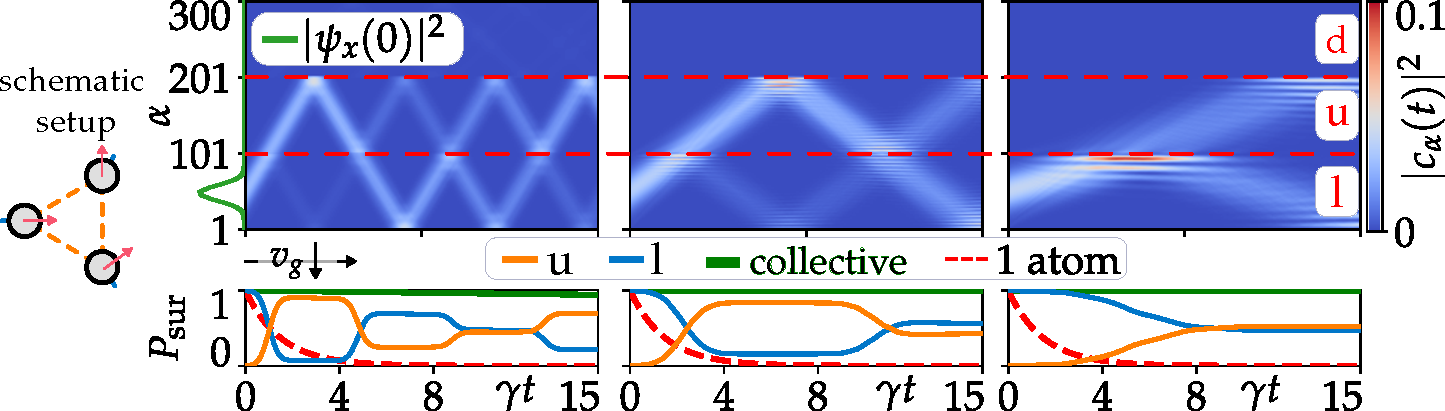
\includegraphics[width=1.0\textwidth]{Topologies_EVO_N_300_v_g}
%    \decoRule
    \caption{Evolution for a system with $ N = 300 $ and an equilateral triangle with unique dipoles.
    The distance is chosen to be \(d \approx 0.05 \lambda \) and the corresponding angles \( \phi_{1,2,3} = [22.12^\circ, 38.56^\circ, 29.68^\circ] \) are extracted from \autoref{fig:Three_Topologies_and_optimization}.
    The same quantities as in \autoref{fig:EVO_Topologies_N_60} are plotted for different initial states.
    The wave packet is centered around $k_\text{s} = 0.43, 0.79, 0.92 \frac{\pi}{d_\text{ext}} $ from left to right and $ \sigma_k = 0.01 \frac{\pi}{d_\text{ext}} $.
    Increasing $k_\text{s}$ reduces the group velocity $ v_\text{g} $.}
    \label{fig:Routing_dep_on_v_g}
\end{figure}

\noindent
As can be seen in \autoref{fig:Routing_dep_on_v_g}, a higher group velocity results in a higher transmission $T$.
As $ k_\text{s} $ increases,
the group velocity $ v_\text{g} $ decreases because the dispersion is less steep at the Brillouin zone boundary $ k = \pm \frac{\pi}{d_\text{ext}} $ (see \autoref{fig:MOM_REAL_SPACE_CHAIN}).
%Generally using a bigger $ k_s $,
%closer to the Brillouin zone boundary $ k = \pm \frac{\pi}{d_\text{ext}} $ results in a smaller group velocity,
%because the dispersion is steeper at the Brillouin zone center.
As a result, the transmission decreases.
However, a higher group velocity and thus higher transmission comes at the cost of a higher dissipation,
which can be seen
since the collective survival probability $P_{\text{sur}}$ decreases faster for lower $ k_{\text{s}}$.
This observation aligns with the fact that the Brillouin zone center corresponds to the superradiant regime (see \autoref{fig:MOM_REAL_SPACE_CHAIN}).

\begin{table}[h!]
\centering
\caption{The dependence of $ k_\text{s} $ on $R$, $T$, and $L$ for $N = 300$ and an equilateral triangle with unique dipoles}
\begin{tabular}{@{}cc@{}}
    % Subfigure containing the figure on the left
    \begin{minipage}{0.22\textwidth}
        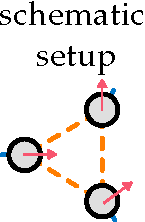
\includegraphics[width=0.5\textwidth]{Topologie_SETUP_N_300_v_g}
    \end{minipage} &
    % The table on the right
    \begin{minipage}{0.78\textwidth}
        \begin{tabular}{@{}lccc@{}}
        \toprule
        \textbf{Case} & \textbf{$ R $} & \textbf{$ T $} & \textbf{$ L $} \\
        \midrule
        \textbf{$k_\text{s} = 0.43 \frac{\pi}{d_\text{ext}}$ ($T = 1 / \gamma$)} & 8.58 & 89.28 & 1.92 \\
        \textbf{$k_\text{s} = 0.79 \frac{\pi}{d_\text{ext}}$ ($T = 3 / \gamma$)} & 15.73 & 84.02 & 0.00 \\
        \textbf{$k_\text{s} = 0.92 \frac{\pi}{d_\text{ext}}$ ($T = 7 / \gamma$)} & 47.62 & 52.28 & 0.00 \\
        \bottomrule
        \end{tabular}
    \end{minipage}
\end{tabular}
\label{tab:coefficients_k_s}
\end{table}

\noindent
Table \ref{tab:coefficients_k_s} presents the reflection, transmission, and leakage coefficients for varying values of $k_\text{s}$.
As $k_\text{s}$ increases, the reflection coefficient ($R$) also increases, while the transmission coefficient ($T$) decreases.
This indicates that a higher group velocity, associated with smaller $k_\text{s}$ favors transmission.

\vspace{1cm}
\noindent
The symmetric topology, the equilateral triangle with unique dipoles, and isosceles triangle, have provided a comprehensive understanding of how the group velocity, atomic distance, and dipole orientations influence the transmission.

\noindent
Having analyzed all factors
that determine the transmission of a photonic excitation on the system of three connected atomic chains,
the overall optimized conditions will now be applied for $N = 300$ atoms.
Therefore, the optimal configurations of the three topologies
as well as the center of the wave packet $ k_{\text{s}}$ are chosen as a balance between low dissipation, robust and fast propagation.
The results are visualized in \autoref{fig:EVO_Topologies}.

\begin{figure}[!ht]
    \centering
    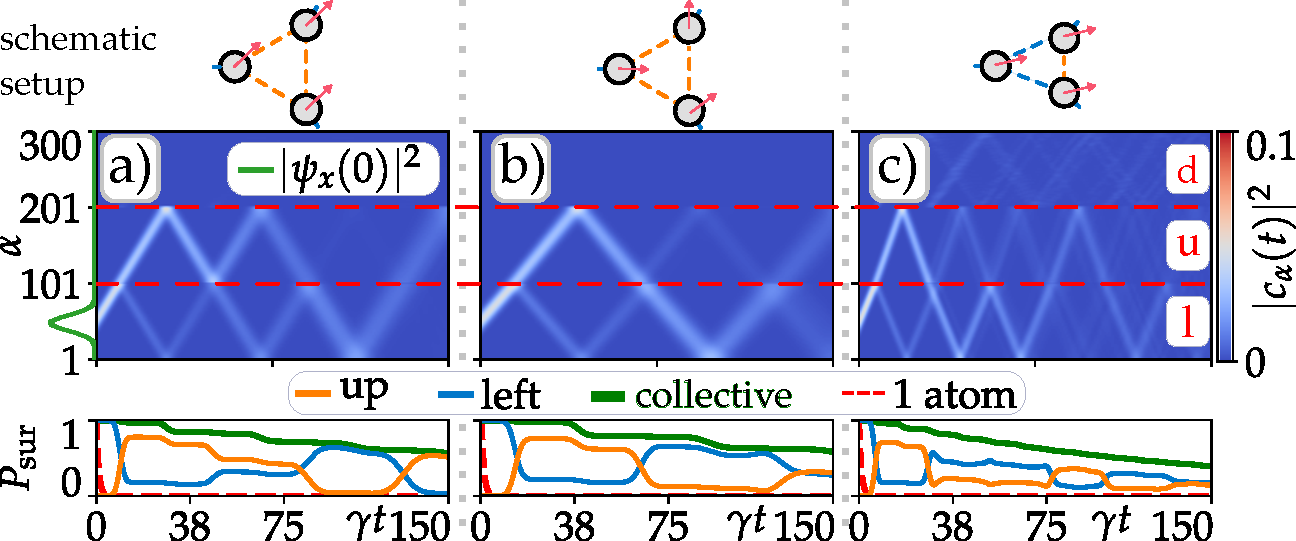
\includegraphics[width=0.8\textwidth]{Topologies_EVO_N_300_final}
    \caption{Evolution for $ N = 300 $ with $ \sigma_k = 0.02 \frac{\pi}{d_\text{ext}} $ and  $k_\text{s} \approx 0.5 \frac{\pi}{d_\text{ext}} $.
    This figure shows similar plots as in Fig.~\ref{fig:EVO_Topologies_N_60}, now for the optimal configurations of \autoref{sec:solutions}:
    \textbf{a)} Symmetric topology with \(\phi_{\text{opt}} = 30.04^\circ\), \(d_{\text{opt}} = 0.12\lambda\), \textbf{b)} Equilateral triangle with unique dipoles \(\phi_{\text{opt,1}} = 32.08^\circ\), \(\phi_{\text{opt,2}} = 29.63^\circ\) and \(\phi_{\text{opt,3}} = 29.12^\circ\), \(d_{\text{opt}} = 0.13\lambda\) and \textbf{c)} Isosceles triangle with aligned dipoles with \(\phi_{\text{opt}} = 31.69^\circ\) and \(d_{\text{opt}} = 0.09\lambda\).}
    \label{fig:EVO_Topologies}
\end{figure}


\noindent
For all triangle types, the wave packet primarily transmits into the upper arm, with variations in reflection into the left arm and leakage into the lower arm.
The reflection ($R$), transmission ($T$), and leakage ($L$) coefficients for each setup are highlighted in \autoref{tab:coefficients_topologies}

\begin{table}[h!]
\centering
\caption{Reflection ($R$), Transmission ($T$), and Leakage ($L$) coefficients for different topologies with $N = 300$ at $k_\text{s} \approx 0.5 \frac{\pi}{d_\text{ext}} $.
    Again, "E" means equilateral geometry, and "I"
    stands for isosceles geometry while "aligned" ("unique") hints at the dipole orientations.}
\begin{tabular}{@{}lccc@{}}
    \toprule
    \textbf{Topology} & \textbf{$R$} & \textbf{$T$} & \textbf{$L$} \\
    \midrule
    E, aligned ($T = 20 / \gamma$) & 17.84 & 78.22 & 1.17 \\
    E, unique ($T = 20 / \gamma$) & 22.30 & 75.68 & 0.04 \\
    I, ligned ($T = 15 / \gamma$) & 17.90 & 70.77 & 7.49 \\
    \bottomrule
\end{tabular}
\label{tab:coefficients_topologies}
\end{table}

\noindent
The equilateral triangle generally exhibits higher transmission and lower reflection compared to the isosceles triangle, with minimal leakage.
In the equilateral triangle, the wave packet components that split at the triangle effectively overlap when they encounter the triangle again.
This results in a more consistent group velocity along each chain, enhancing overall transmission and reducing leakage.
Each encounter with a chain's edge results in a small dip in survival probability, similar to a single chain scenario.
For the isosceles triangle, these dips occur more frequently, reducing the survival probability over time.
The smaller atomic distances of the chain $ d_\text{ext} $ in this topology increase the group velocity, leading to more reflections and consequently higher losses.
This results in the lowest survival probability among the topologies studied, with notable leakage into the lower arm.
The completely symmetric topology demonstrates the highest stability, with no significant leakage and a relatively high transmission coefficient.
The setup with unique dipole orientations offers similarly good results.
However, it is not physically achievable in practice.
Therefore, the equilateral triangle with aligned dipoles is more relevant for stable readout.
The isosceles triangle is suitable for faster readout at the cost of an increased leakage.
\chapter{Conclusion}
\label{Chapter5}
%----------------------------------------------------------------------------------------
%	SECTION 1
%----------------------------------------------------------------------------------------
This thesis explored the feasibility of directional routing of excitations in atomic systems using subradiant states.
Bottarelli's abstract quantum router model was adapted to an atomic system.
In this adaptation, a phase $ \theta $ was found that resembles the phase in the loop of Bottarelli's work.
It depends on atomic distances and dipole orientations.
However, this phase proved to be insufficient for achieving directional routing.
This was due to the non-Hermitian nature of the Hamiltonian governing the complex open system dynamics, which does not exhibit chirality.
The challenges of controlling interactions in fully connected setups were also discussed.
Consequently, it was necessary to modify Bottarelli's original approach to achieve effective routing.

\noindent
By changing both the atomic distance and dipole orientations, three different triangular topologies were investigated:
The equilateral triangle with aligned dipoles,
the equilateral triangle with unique dipoles, and the isosceles triangle with aligned dipoles.
It was shown that controlling the setup allows for a "brute-force"
directional routing of excitations in the atomic system by minimizing specific dipole-dipole couplings in the triangle.

\noindent
The topology with unique dipole orientations showed a very high transmission coefficient of $ T \approx 90 $ for very closely spaced atoms $d_\text{ext} = d = 0.05 \lambda$.
But this setup is hard to prepare experimentally as one would need an inhomogeneous external field applied to the apparatus.
The routing for the optimal distances around $ d_\text{ext} = 0.1 \lambda $ was demonstrated to be most effective
when the initial wave packet is centered at $k_\text{s} \approx \pi / (2 d_{\text{ext}})$ where a balance between low dissipation,
robust and fast propagation was achieved.
The equilateral triangle with aligned dipoles emerges as the most viable solution for stable transmission of $ T \approx 78 $ in experimental setups,
fitting with Bottarelli's original topology.

\noindent
For larger atomic systems, routing effectiveness improved.
The results also suggest that an isosceles triangle is suited for faster readout,
though this comes at the cost of higher leakage into the unwanted chain.


\noindent
In summary, this work provided a framework for achieving directional routing in atomic systems.
Future research could investigate the implementation of these findings in experimental conditions.
It would also be interesting to see whether similar directional routing can be achieved in systems with multiexcitation states.

%----------------------------------------------------------------------------------------
%	APPENDICES
%----------------------------------------------------------------------------------------

\appendix
% Appendix A

\chapter{Extra material} % Main appendix title

\label{AppendixA} % For referencing this appendix elsewhere, use \ref{AppendixA}

%-----------------------------------
%	SECTION 1
%-----------------------------------
\section{Phase Problem} \label{sec:No_direcionality}
This section shows that a problem with the correspondence of a phase to an evolution exists.
It arises when Bottarelli's approach is directly implemented on an atomic system in \autoref{sec:challenges}.

\noindent
For $ N = 6 $ one can recreate the topology as in \autoref{fig:botarellis_topo}.
The phase $ \theta $ depends on the positions and dipole orientations of the three loop-atoms.
This dependence is shown in \autoref{fig:Theta_vs_d_phi_different_Evo} a).
Multiple combinations that lead to the same $ \theta $ have different evolutions,
which is depicted in \autoref{fig:Theta_vs_d_phi_different_Evo} b).
\begin{figure}[ht]
    \centering
    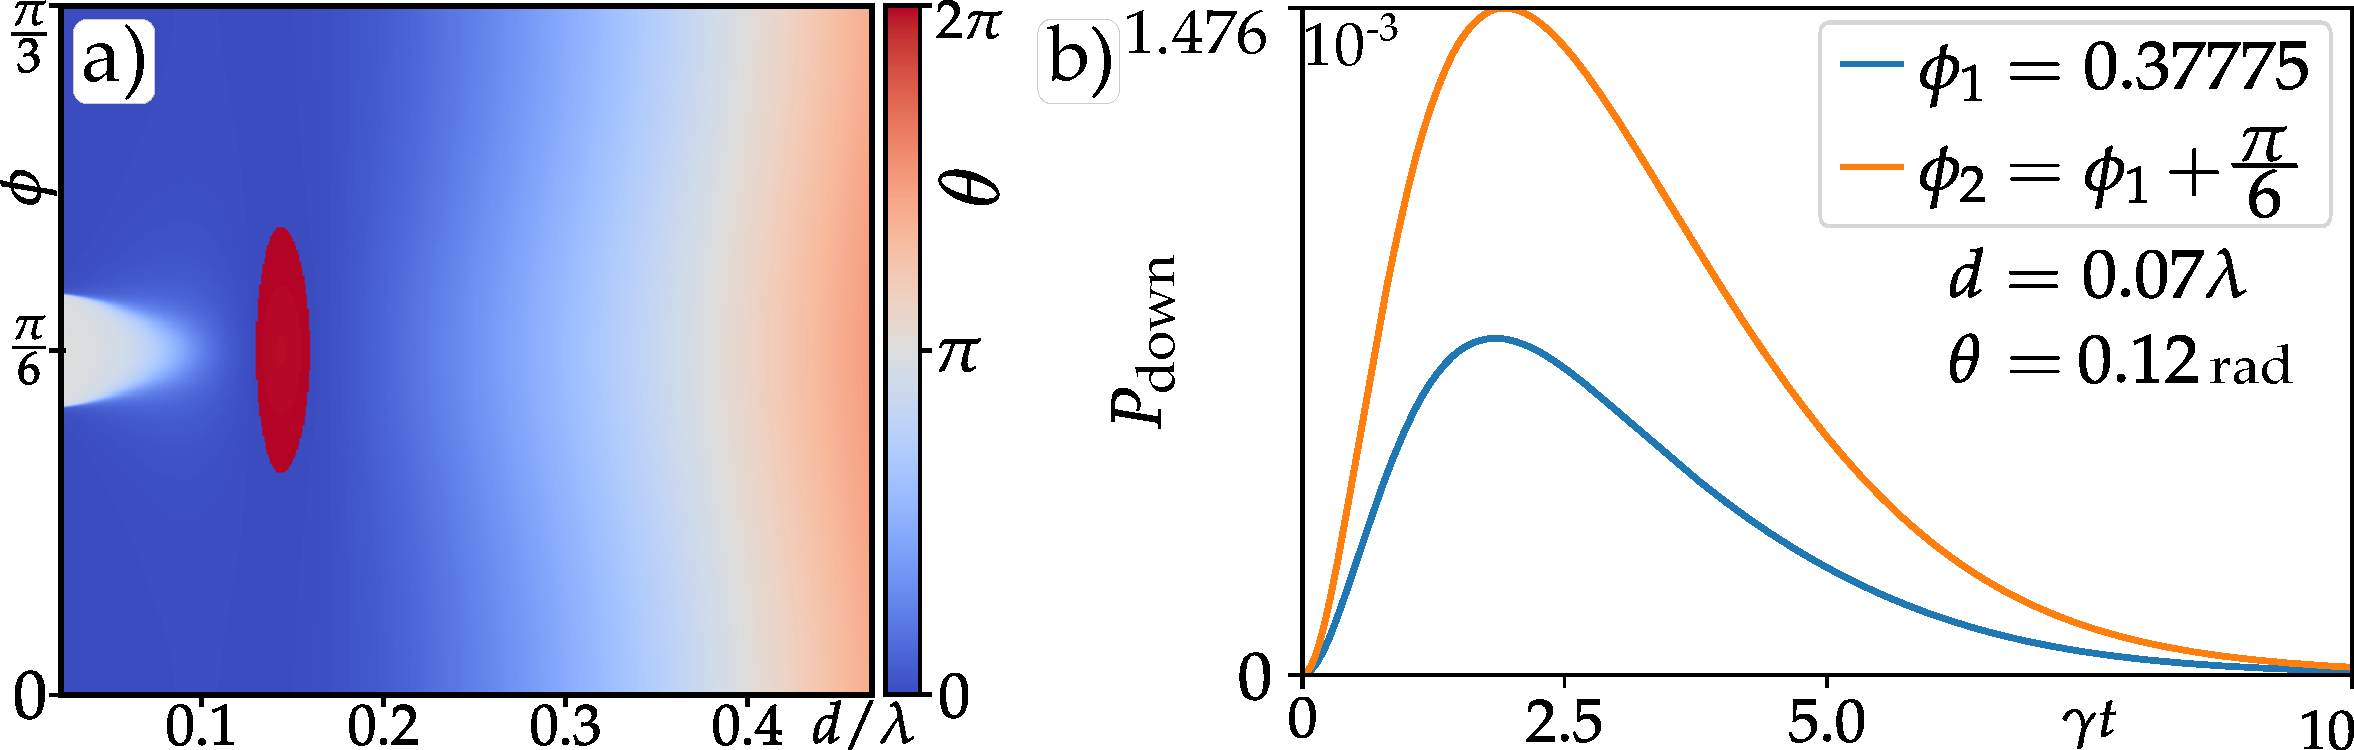
\includegraphics[width=\textwidth]{THETA(d,angle)_for_all_inner}
    \caption{The first plot (a) Shows the dependence of the phase in the loop for an equilateral triangle.
    The angle $ \phi $ measures the orientation of the dipoles with respect to the x-axis.
    Care must be taken, as multiple combinations of $d/\lambda$ and $ \phi $ can lead to the same $ \theta $ but result in different evolutions, as seen in (b).
    The second plot (b) shows the evolution of a classical state which is initially on the left arm, exactly like in \cite{Startingpoint}.}
    \label{fig:Theta_vs_d_phi_different_Evo}
\end{figure}
But again, changing the phase does not allow for directional routing in the first place.
The Hamiltonian for the atomic system is not hermitian and chirality is not possible.

\newpage
%-----------------------------------
%	SECTION 2
%-----------------------------------
\section{Diagonalization} \label{sec:Diagonalization}
The Hamiltonian of a infinite system can be diagonalized with a Fourier transformation.
This section shows that it is still useful to operate in $k$-space even for a finite system, as mentioned in section \ref{sec:Sys_def_N_bigger_6}.

\noindent
The matrices $ V $ and $ \Gamma $ described in section \ref{sec:Single_Excitation}, can be approximately diagonalized
using the Fourier transformation from Eq. \eqref{eq:FT}.
\autoref{fig:Diagonalizable} displays these matrices in both real- and reciprocal-space basis.
In $k$-space they are primarily diagonal with a small defect in the off-diagonal corners.
Increasing the number of atoms reduces the extent of this defect.

\begin{figure}[ht]
    \centering
    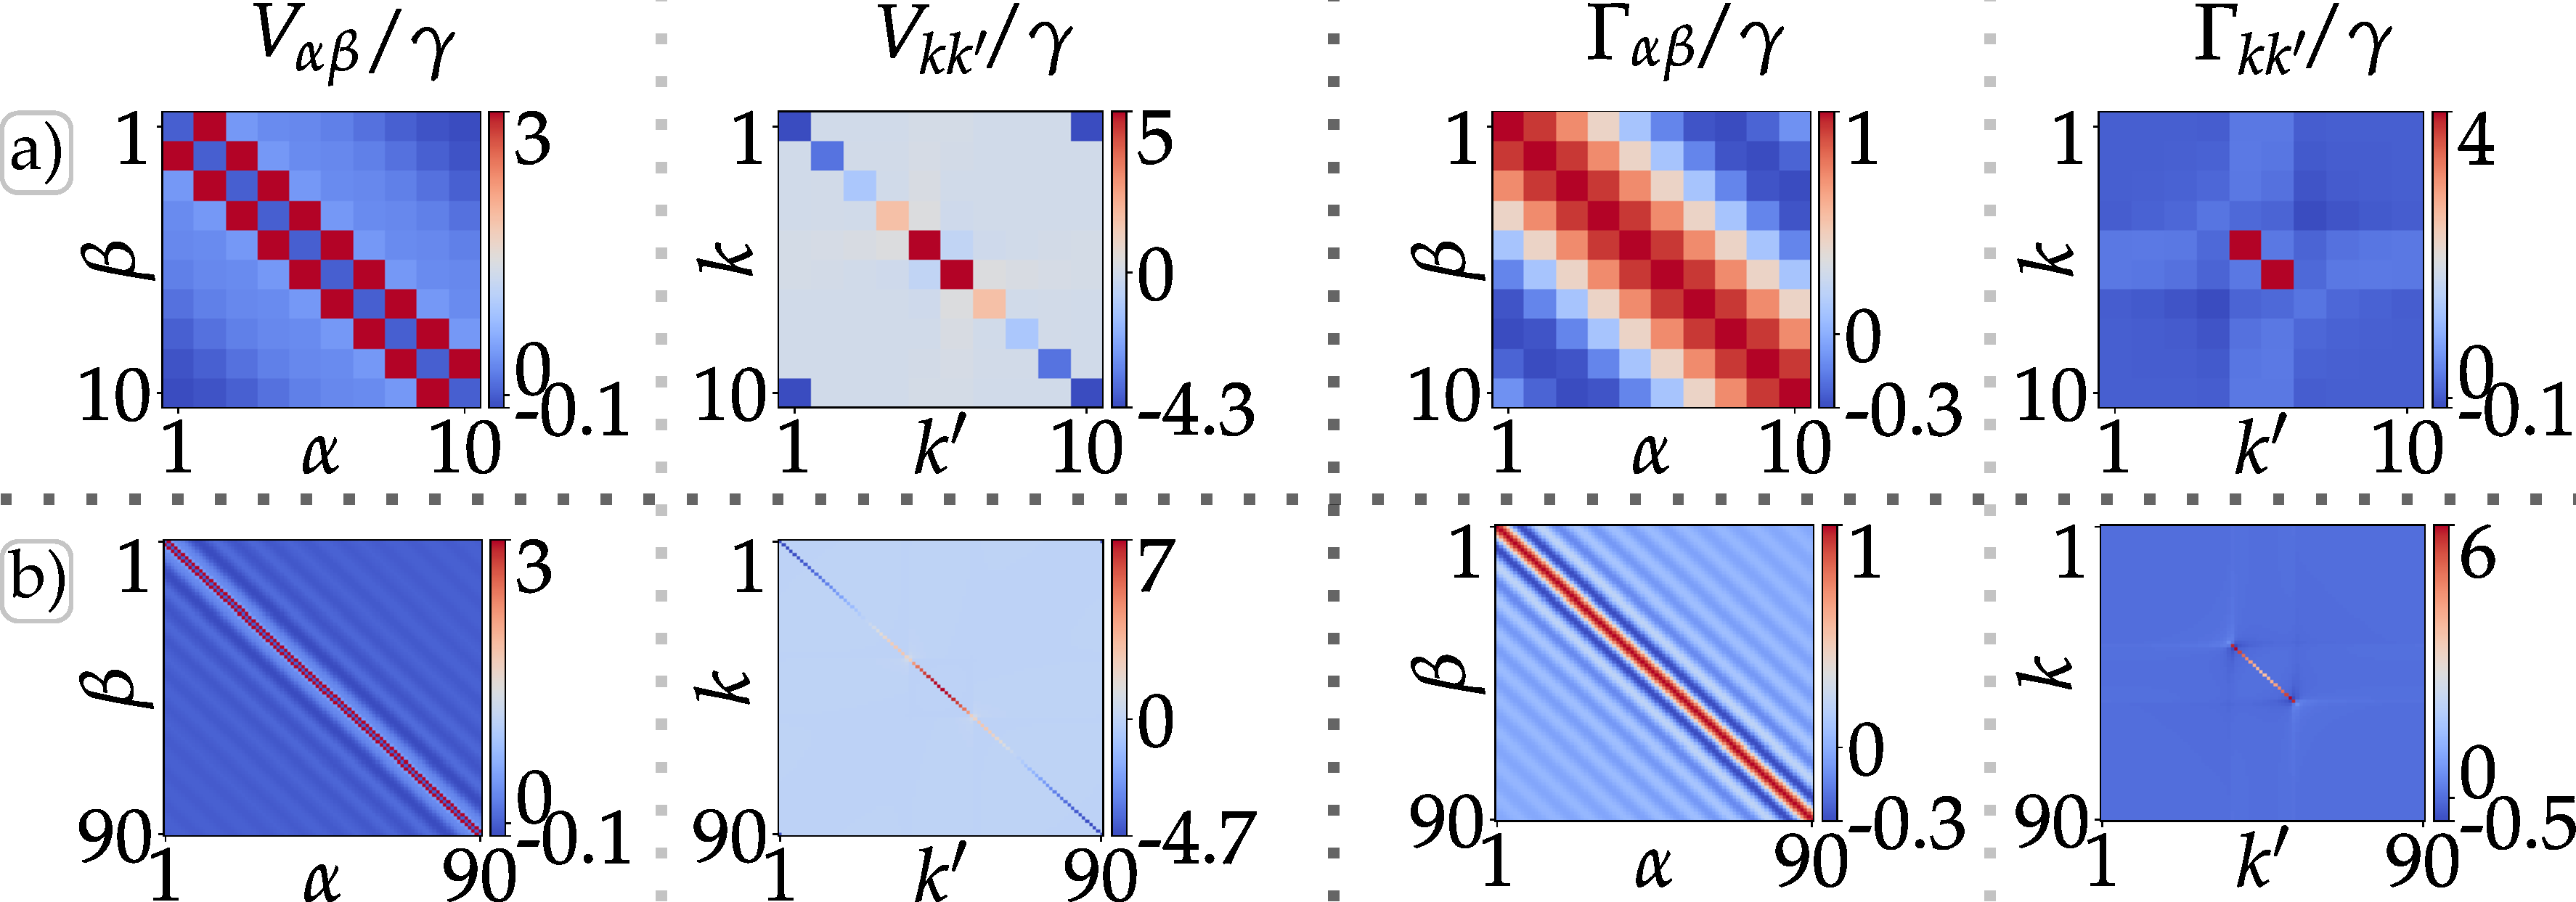
\includegraphics[width=1.0\textwidth]{V_matrix_Real_and_k_space}
    \caption{\textbf{a)} Chain of $N = 10 $ atoms.
    \textbf{b)} Chain of $N = 90 $ atoms.
    The atomic dipoles are aligned and perpendicular to the chain, and the interatomic distance is chosen to be $ d = 0.1 \lambda $.
    The interaction matrix $ (V)_{\alpha \beta} $ and $ (\Gamma)_{\alpha \beta} $ are displayed in units of $ \gamma $.
    Left side in real space and right side in $k$-space.}
    \label{fig:Diagonalizable}
\end{figure}

%----------------------------------------------------------------------------------------
%	BIBLIOGRAPHY
%----------------------------------------------------------------------------------------

\printbibliography

\end{document}